\documentclass[conference,10pt]{IEEEtran}

\usepackage{silence}
\WarningFilter{latexfont}{Font shape}
\WarningFilter{latexfont}{Size substitutions}
\usepackage{amsmath,amssymb,amsfonts,amsthm}
\usepackage{algorithmic}
\usepackage{algorithm}
\usepackage{array}
\usepackage{booktabs}
\usepackage{cite}
\usepackage{graphicx}
\usepackage{textcomp}
\usepackage{xcolor}
\usepackage{url}
\usepackage{tikz}
\usepackage{pgfplots}
\pgfplotsset{compat=1.18}

\setlength{\emergencystretch}{3em}
\hbadness=10000
\vbadness=10000

\newtheorem{theorem}{Theorem}
\newtheorem{lemma}[theorem]{Lemma}
\newtheorem{definition}{Definition}
\newtheorem{corollary}[theorem]{Corollary}
\newtheorem{invariant}{Invariant}

\hyphenation{op-tical net-works semi-conduc-tor}

\begin{document}

\title{Hardware-Aware Speculative KV-Cache Paging and Epistemic Attention Eviction for High-Throughput Multi-Turn Agentic LLM Serving}

\author{
\IEEEauthorblockN{Aniket Agrawal}
\IEEEauthorblockA{Cloud Engineer, Google Cloud \\
Google, Bangalore, India \\
aniketagrawal@google.com}
}

\maketitle

\begin{abstract}
The rapid proliferation of autonomous multi-turn agentic workflows has exacerbated the memory capacity bottleneck in Large Language Model (LLM) inference accelerators. In modern agentic sequences spanning $32\text{k}$ to $128\text{k}+$ tokens ($L=64, H_{\text{kv}}=8, d_k=128$, \texttt{float16}), Key-Value (KV) cache memory footprints expand to $17.18\text{ GB}$ ($16.00\text{ GiB}$) per active $64\text{k}$-token agent stream ($8.59\text{ GB}$ / $8.00\text{ GiB}$ at $32\text{k}$ tokens). Even under multi-chip tensor-parallel weight and KV-cache sharding or $32\text{k}\text{--}64\text{k}$ context distributions, this memory demand precipitates an acute capacity cliff on accelerators such as the Google Cloud TPU v6e Trillium (32~GB HBM per chip), exhausting non-weight HBM capacity after only 3 to 8 concurrent sequences. Existing virtualized inference engines (e.g., PagedAttention / vLLM and SGLang / RadixAttention) mitigate Out-Of-Memory exceptions via reactive demand paging to Host DRAM over PCIe/CXL. However, servicing a synchronous full-layer demand page fault ($64 \times 64\text{ KiB} = 4\text{ MiB}$ across $L=64$ layers, or $1.87\,\mu\text{s}$ of raw wire serialization per single-layer $64\text{ KiB}$ block at $35\text{ GB/s}$ effective PCIe Gen5 bandwidth plus descriptor ring wakeup and dirty writeback) incurs severe pipeline stalls ($0.12\text{ ms}$ to $0.50\text{ ms}$ per faulted step against $0.16\text{ ms}$ ideal compute), causing matrix execution units to idle for 40\% to 70\% of execution time. Furthermore, classical page eviction policies (LRU/LFU) are attention-blind: they inadvertently evict initial prompt attention sinks and active tool schemas while preserving ephemeral chain-of-thought scratchpad tokens.

To overcome these constraints, we present \textbf{Speculative Epistemic KV-Cache Paging (SE-Paging)} governed by the \textbf{Epistemic Least-Likely-Attended (ELLA)} eviction protocol. SE-Paging couples the agent's semantic execution graph and turn-smoothed epistemic branch entropy $\mathcal{H}_i(t)$ to physical memory management: (1) an Epistemic Working Set Estimator (EWSE) projects future attention mass $\mathcal{A}(P_k, t)$, permanently pinning attention sinks and retaining active/idle tool schemas and DAG-boosted history while decaying idle tool schemas below DAG-predicted history within $\approx 8$ steps ($\approx 1$ turn) and aggressively evicting resolved scratchpad pages; (2) an Asynchronous DMA Speculative Prefetcher (ADSP) with sealed-page write-through host mirroring overlaps Host-to-Device page transfers with active matrix computation across a $\tau_{\text{lookahead}}=2$-step horizon; and (3) ELLA establishes bounded competitive ratios relative to offline Belady MIN under both non-cascading trace-regular greedy eviction and randomized Predictive Marker phases. We evaluate SE-Paging in a downscaled $1:32$ trace-driven CPU-based physical tensor-buffer memory-hierarchy emulator (modeling a 2-layer $128\text{ KiB}$ slice per $B=16$-token page, $N_{\text{dev}}=96$ HBM pages [$12.00\text{ MiB}$], $N_{\text{host}}=2{,}500$ DRAM pages [$312.50\text{ MiB}$], and $976$ allocated physical pages [$16$ shared prefix + $48$ private pages/stream, or $15{,}616$ total tokens] across $K=20$ streams) parameterized to scaled TPU v6e Trillium and PCIe Gen5 timing, complemented by a 6-turn live trace replay on Google Cloud Vertex AI (\texttt{gemini-2.5-flash}) and parameterized multi-turn SWE-bench and Gorilla API emulation traces. Across $5{,}940$ logical page-lookup cycles ($11{,}880$ two-stage memory-subsystem operations per protocol) spanning $K \in \{4, 8, 12, 16, 20\}$ concurrent agent streams under $10.17\times$ physical ($13.33\times$ unshared logical) working-set overflow, SE-Paging elevates cache hit rate at $K=20$ from 0.20\% (LRU) and 1.21\% (LFU) to \textbf{28.23\%} ($28.31 \pm 0.38\%$ 5-seed mean), retains \textbf{98.64\%} empirical Query-Key (QK) RoPE dot-product attention mass, eliminates 46.8\% of memory pipeline stall overhead, and increases simulated device throughput by 49.3\% (+53.4\% in host wall-clock page-lookup throughput) over LRU.
\end{abstract}

\begin{IEEEkeywords}
KV-Cache Memory Management, Hardware Accelerators, TPU v6e Trillium, Speculative DMA Prefetching, Multi-Agent LLM Serving, PagedAttention, Virtual Memory.
\end{IEEEkeywords}

\section{Introduction}
\IEEEPARstart{E}{nterprise} deployment of autonomous agent swarms built on foundation models (e.g., Gemini 2.5 Pro/Flash, Gemma 2, and Claude) represents a major workload shift in cloud computing. In frameworks such as the Google Agent Development Kit (ADK) and Vertex AI Agent Builder, agents engage in prolonged, multi-turn reasoning workflows involving hierarchical sub-goal decomposition, external tool invocations via OpenAPI schemas~\cite{patil2024gorilla}, and structured artifact generation~\cite{zheng2024sglang, gao2024cachedattention}.

\subsection{The KV-Cache HBM Capacity Cliff}
Unlike traditional stateless NLP classification or single-turn dialogue, agentic sequences accumulate extensive conversational histories, tool schemas, and chain-of-thought scratchpads, routinely expanding context lengths from $32\text{k}$ to $128\text{k}+$ tokens~\cite{kwon2023efficient, xiao2023efficient}.

During auto-regressive transformer decoding, Key and Value activation vectors for every past token must remain memory-resident to avoid redundant quadratic recomputation. The physical memory required scales linearly with context length $S$, transformer layers $L$, KV heads $H_{\text{kv}}$, and head dimension $d_k$:
\begin{equation}
\label{eq:kv_footprint}
\text{Memory}_{\text{KV}} = 2 \times L \times H_{\text{kv}} \times d_k \times S \times \text{bytes\_per\_elem}
\end{equation}
For a representative enterprise model ($L=64$, $H_{\text{kv}}=8$, $d_k=128$, \texttt{float16} with $\text{bytes\_per\_elem}=2$), a sequence of $S = 64\text{k} = 65{,}536$ tokens requires $17{,}179{,}869{,}184\text{ bytes} \approx \mathbf{17.18\text{ GB}}$ decimal ($\mathbf{16.00\text{ GiB}}$ binary) of dedicated High-Bandwidth Memory (HBM) (or $8{,}589{,}934{,}592\text{ bytes} \approx \mathbf{8.59\text{ GB}}$ decimal / $\mathbf{8.00\text{ GiB}}$ binary for $S = 32\text{k} = 32{,}768$ tokens).

On modern cloud accelerators such as the Google Cloud TPU v6e Trillium (configured with 32~GB HBM in 256-chip 2D torus pods, following Google's custom TPU architectures~\cite{jouppi2023tpu}) or GPU nodes~\cite{sheng2023flexgen}, this memory demand triggers an immediate \textit{capacity cliff}: even under multi-chip tensor-parallel model-weight and KV-cache sharding (where 64-layer weights are partitioned across chips, leaving $12\text{--}24\text{ GiB}$ of non-weight HBM per chip) or $32\text{k}\text{--}64\text{k}$ context distributions with shared prefixes, a chip exhausts its remaining HBM pool after serving only 3 to 8 concurrent agent sequences, capping cluster concurrency.

\subsection{The Demand Paging Pipeline Stall Dilemma}
To prevent fatal Out-Of-Memory (OOM) aborts, modern serving runtimes (e.g., vLLM / PagedAttention~\cite{kwon2023efficient} and SGLang~\cite{zheng2024sglang}) partition the KV-cache into discrete non-contiguous physical pages ($B = 16$ tokens per block) and implement reactive \textit{demand swapping} to Host DRAM over PCIe Gen5 or CXL, while multi-turn offloading systems such as CachedAttention~\cite{gao2024cachedattention} perform coarse-grained inter-turn session pre-loading across conversation boundaries.

However, intra-turn demand swapping is fundamentally reactive: when the accelerator's matrix execution units encounter an unmapped page during token generation, the decoding pipeline stalls. Over a PCIe Gen5 $\times 16$ interconnect ($64\text{ GB/s}$ theoretical unidirectional bandwidth, $\approx 35\text{ GB/s}$ effective under multi-stream contention), transferring a single-layer $64\text{ KiB}$ page block ($B=16, H_{\text{kv}}=8, d_k=128$) requires $\approx 1.87\,\mu\text{s}$ of raw wire serialization ($3.74\,\mu\text{s}$ per fused 2-layer $128\text{ KiB}$ slice, or $119.7\,\mu\text{s}$ across all $L = 64$ transformer layers totaling $4\text{ MiB}$ per 16-token block); combined with PCIe DMA descriptor ring wakeup and synchronous dirty-page writeback, a full-model page fault stalls token generation for \textbf{$0.12\text{ ms}$ to $0.50\text{ ms}$} ($0.288\text{--}0.384\text{ ms}$ in our calibrated parameterization vs.\ $0.160\text{ ms}$ ideal 64-layer compute)~\cite{sheng2023flexgen, lee2024infinigen}. Under high sequence concurrency, these synchronous demand stalls accumulate, causing matrix execution units to spend \textbf{40\% to 70\% of wall-clock time stalled waiting on memory}.

\subsection{The Attention-Blind Eviction Failure}
Furthermore, classical operating system page eviction policies (Least Recently Used [LRU], Least Frequently Used [LFU], FIFO) and existing token-pruning or single-step rehearsal heuristics are mismatched with multi-turn agentic transformer physics:
\begin{enumerate}
    \item \textbf{Destruction of Attention Sinks and Tool Schemas:} Transformers concentrate massive attention mass on the initial 1 to 4 sink blocks~\cite{xiao2023efficient} and active OpenAPI tool definitions~\cite{patil2024gorilla}. Under LRU, as an agent generates thousands of intermediate reasoning tokens, initial prompt tokens and tool schemas are aged out to Host RAM. While static window methods like StreamingLLM~\cite{xiao2023efficient} drop middle tokens permanently, Heavy-Hitter Oracle (H2O)~\cite{zhang2023h2o} tracks cumulative attention scores, Quest~\cite{tang2024quest} estimates page criticality from query-key bounding boxes within the current layer without multi-step DMA prefetching, and InfiniGen~\cite{lee2024infinigen} performs single-step layer-adjacent rehearsal prefetching (using skewed query-key projections in layer $l-1$ to prefetch layer $l$), none of these approaches satisfy multi-step PCIe lookahead horizons ($\tau_{\text{lookahead}} = 2$ steps ahead) during abrupt multi-turn agentic tool-call DAG transitions where an entire dormant tool schema or prior history segment suddenly regains high query-key attention alignment. Similarly, unlike purely static agentic workflow prefetchers (KVFlow~\cite{pan2025kvflow}) or prefix-tree LRU schedulers (SGLang / RadixAttention~\cite{zheng2024sglang}) that ignore live generation uncertainty, SE-Paging couples workflow DAG lookahead with turn-smoothed epistemic Shannon entropy $\mathcal{H}_i(t)$.
    \item \textbf{Scratchpad Memory Pollution:} Intermediate chain-of-thought scratchpad tokens are predominantly transient: once an agent concludes a reasoning sub-step, its scratchpad tokens carry rapidly decaying query-key weight unless backtracking occurs. Classical LRU retains newly written scratchpad pages in fast HBM, displacing reusable history and tool schemas.
\end{enumerate}

\subsection{Contributions}
In this paper, we propose \textbf{Hardware-Aware Speculative KV-Cache Paging (SE-Paging)} governed by the \textbf{Epistemic Least-Likely-Attended (ELLA)} eviction protocol. Our key contributions are:
\begin{enumerate}
    \item \textbf{Epistemic Working Set Estimator (EWSE):} A formal priority formulation that projects future page attention mass $\mathcal{A}(P_k, t)$ from agent semantic segment tags, stream-indexed tool-call and history DAG lookahead $\hat{d}_{\text{DAG},i}(P_k, t)^{-1}$, and conditionally re-normalized action-delimiter epistemic Shannon entropy $\mathcal{H}_i(t)$.
    \item \textbf{Asynchronous DMA Speculative Prefetcher (ADSP):} A non-blocking prefetcher restricted to lookahead-predicted non-resident candidates with sealed-page write-through host mirroring that dispatches Host-to-Device transfers at step $t = n - \tau_{\text{lookahead}}$, overlapping PCIe/CXL transfer latency with matrix compute while eliminating synchronous dirty-page writebacks.
    \item \textbf{Theoretical Performance Guarantees:}
    \begin{itemize}
        \item \textbf{Theorem 1 (Queued Zero-Stall Pipeline Overlap):} Establishes the step-indexed multi-page lookahead condition $\tau_{\text{lookahead}} \ge \left\lceil \frac{M_{\text{pre}}(n) T_{\text{DMA}}(P_k)}{(1-\rho_{\text{bus}})T_{\text{compute}}} \right\rceil$ under an unbacklogged or steady-state stable DMA queue under which device stall cycles are identically zero.
        \item \textbf{Theorem 2 (Attention Mass Preservation):} Proves that ELLA scratchpad eviction beyond the pinned active window ($\delta = 64$ tokens) of the executing stream analytically bounds attention mass loss by $\epsilon_{\text{attn}} \le C\delta^{1-\gamma}\!\left(\frac{1}{\delta} + \frac{1}{\gamma-1}\right) \le \frac{C_{\text{scratch}}}{(\gamma - 1)\delta^{\gamma - 1}}$ ($\le 0.0261$ at $\delta=64$ and $\le 0.0105$ at $\delta=256$ from the intermediate integral bound), complemented by non-circular empirical Query-Key (QK) RoPE softmax attention evaluation showing $98.64\%$ retained attention mass ($96.80\%$ top-$k$ QK page recall).
        \item \textbf{Theorem 3 (Bounded Competitive Ratio):} Uses the competitive caching with predictions framework~\cite{lykouris2021competitive} on acyclic agentic execution graphs to establish expected competitive ratios of $\mathbb{E}[\mathcal{C}_{\text{ELLA}}^{\text{greedy}}] \le 1 + \mathcal{O}(\eta_{\text{tot}}/\text{OPT} + \mathcal{H}_{\max})$ under non-cascading trace-regular greedy eviction and $\mathbb{E}[\mathcal{C}_{\text{ELLA}}^{\text{marker}}] \le 2 + \mathcal{O}(\min(\sqrt{\mathbb{E}[\eta_{\ell_1}]/\text{OPT}}, \log N_{\text{dev}}))$ when paired with randomized Predictive Marker phases relative to offline Belady MIN~\cite{belady1966study}.
    \end{itemize}
    \item \textbf{Downscaled Physical Tensor-Buffer Emulator, Multi-Turn Benchmark Generalization \& Live Vertex AI Trace Replay:} We evaluate SE-Paging in a downscaled $1:32$ CPU-based physical tensor-buffer emulator (modeling a 2-layer $128\text{ KiB}$ slice per page, $N_{\text{dev}}=96$ HBM pages [$12.00\text{ MiB}$], $N_{\text{host}}=2{,}500$ DRAM pages [$312.50\text{ MiB}$], and $976$ allocated physical pages [$16$ shared prefix + $48$ private pages/stream, or $15{,}616$ total tokens] across $K=20$ streams) across $5{,}940$ logical page-lookup cycles ($11{,}880$ two-stage memory-subsystem operations per protocol), comparing against 11 baseline and ablation configurations (\texttt{DEMAND\_LRU}, \texttt{DEMAND\_LFU}, \texttt{SGLang/RadixAttention}~\cite{zheng2024sglang}, \texttt{StreamingLLM}~\cite{xiao2023efficient}, \texttt{H2O}~\cite{zhang2023h2o}, \texttt{Quest}~\cite{tang2024quest}, \texttt{CachedAttention}~\cite{gao2024cachedattention}, \texttt{InfiniGen}~\cite{lee2024infinigen}, \texttt{DEMAND\_ELLA} with and without write-through mirroring, and \texttt{STATIC\_DAG\_ELLA}~\cite{pan2025kvflow}), plus a $\pm 50\%$ hyperparameter sensitivity study, parameterized multi-turn SWE-bench~\cite{jimenez2024swebench} and Gorilla~\cite{patil2024gorilla} emulation traces, and a 6-turn live Google Cloud Vertex AI (\texttt{gemini-2.5-flash}) trace replay.
\end{enumerate}

\section{Related Work}
\begin{itemize}
    \item \textbf{Virtualized KV-Cache and Offloading Systems:} PagedAttention / vLLM~\cite{kwon2023efficient} introduced OS-inspired block-level KV-cache virtualization ($B=16$ tokens) with reactive demand swapping, while SGLang~\cite{zheng2024sglang} introduced RadixAttention for shared prefix-tree reuse with LRU leaf eviction. FlexGen~\cite{sheng2023flexgen} formulated static linear-programming offload schedules across GPU, CPU DRAM, and disk for offline batch throughput, and CachedAttention~\cite{gao2024cachedattention} overlapped inter-turn session restoration across multi-turn conversation boundaries. However, none of these systems prevent intra-turn page-fault stalls when an active agent dynamically switches between tool schemas and history blocks across sub-steps.
    \item \textbf{Token Pruning and Intra-Layer Sparse Attention:} StreamingLLM~\cite{xiao2023efficient} retains initial attention sinks plus a static sliding window while permanently discarding middle tokens. H2O~\cite{zhang2023h2o} evicts tokens with low cumulative attention scores, Quest~\cite{tang2024quest} selects top-$k$ pages per layer using query-key bounding boxes without asynchronous Host-to-Device DMA lookahead, and InfiniGen~\cite{lee2024infinigen} prefetches KV entries from layer $l-1$ to layer $l$ via skewed projections. While effective for single-step layer overlap, single-layer lookahead ($\tau=1$ layer) is insufficient to hide multi-page PCIe Gen5 transfer latency across multi-turn agentic state transitions.
    \item \textbf{Agent-Aware KV-Cache Management:} Recent agentic serving frameworks such as KVFlow~\cite{pan2025kvflow} and SGLang~\cite{zheng2024sglang} exploit static agentic workflow graphs or radix trees to pre-warm or pin agent prefixes during structured tool-calling workloads~\cite{patil2024gorilla, jimenez2024swebench}. However, static DAG distances are deterministic: when an agent encounters high epistemic branching uncertainty during reasoning or tool error recovery, static schedules either evict active scratchpad context prematurely or fail to adjust history retention dynamically. SE-Paging bridges this gap by combining fine-grained categorical page tagging ($\mathcal{P}_{\text{anchor}}, \mathcal{P}_{\text{tool}}, \mathcal{P}_{\text{active}}, \mathcal{P}_{\text{hist}}, \mathcal{P}_{\text{scratch}}$) and stream-indexed forward DAG distance $\hat{d}_{\text{DAG},i}(P_k, t)^{-1}$ with live turn-smoothed epistemic branch entropy $\mathcal{H}_i(t)$ and sealed-page write-through DMA mirroring.
\end{itemize}

\section{System Architecture and Memory Hierarchy}

\subsection{Heterogeneous Memory Hierarchy Model}
We model an AI inference accelerator node (e.g., Google Cloud TPU v6e Trillium programmed via JAX/Pallas kernels~\cite{bradbury2018jax}) comprising two memory tiers:
\begin{itemize}
    \item \textbf{Tier 0 (Device HBM):} High-bandwidth, capacity-constrained memory directly attached to Matrix Execution Units (MXUs) ($\text{BW}_{\text{HBM}} \ge 1.6\text{ TB/s}$, capacity $C_{\text{HBM}} \in \{32, 64\}\text{ GB}$).
    \item \textbf{Tier 1 (Host DRAM / CXL):} High-capacity system memory connected via PCIe Gen5 / CXL ($\text{BW}_{\text{bus}} \approx 32\text{--}64\text{ GB/s}$, capacity $C_{\text{Host}} \ge 512\text{ GB}$).
\end{itemize}

KV-cache is managed in fixed-size physical page blocks $P_k$ containing $B = 16$ tokens. For a single transformer layer ($H_{\text{kv}}=8, d_k=128$, \texttt{float16}), each page block occupies:
\begin{equation}
\label{eq:page_size}
\begin{aligned}
\text{Size}_{\text{1-layer}}(P_k) &= B \times 2 \times H_{\text{kv}} \times d_k \times 2\text{ bytes} \\
&= 65{,}536\text{ bytes } (64\text{ KiB})
\end{aligned}
\end{equation}
In our multi-layer block allocator (Section~VI-A), pairs of adjacent transformer layers are co-allocated into fused $128\text{ KiB}$ ($131{,}072\text{ byte}$) physical transfer units to amortize PCIe DMA descriptor ring overhead while permitting layer-pipelined DMA interleaving and sub-stack preemption across concurrent streams without blocking on a monolithic $4\text{ MiB}$ transfer. In a full 64-layer deployment, the 32 fused 2-layer slices of logical block $P_k$ share a single logical page-table descriptor and priority score $\mathcal{A}(P_k, t)$ equipped with a 32-bit layer-residency bitmap (\texttt{slice\_mask}); if sub-stack preemption interrupts a 64-layer transfer after slice $s < 32$, layers $1\dots 2s$ execute while the remaining slices resume at the head of the DMA queue prior to layer $2s+1$, and partially resident blocks ($0 < \text{popcount}(\text{slice\_mask}) < 32$) remain pinned in $\mathcal{P}_{\text{pinned\_prefetch}}$ until all 32 slices complete so partially populated blocks are never prematurely evicted. In our scaled $1:32$ slice emulator (modeling a representative 2-layer $128\text{ KiB}$ slice out of $L=64$ layers), per-slice raw DMA wire transfer latency $T_{\text{DMA}}(P_k) = 3.74\,\mu\text{s}$ ($4.56\,\mu\text{s}$ effective slice transfer latency under $\rho_{\text{bus}} = 0.18$ background bus contention), per-slice ideal matrix compute time $T_{\text{compute}}^{\text{ideal}} = 5.00\,\mu\text{s}$, and scaled descriptor wakeup / writeback penalties ($T_{\text{wakeup}} = 4.44\,\mu\text{s}$, $T_{\text{wb}} = 3.00\,\mu\text{s}$, yielding $4.44 + 4.56 = 9.00\,\mu\text{s}$ per clean slice fault or $288.0\,\mu\text{s}$ across 64 layers, and $4.44 + 4.56 + 3.00 = 12.00\,\mu\text{s}$ per dirty slice fault or $384.0\,\mu\text{s}$ across 64 layers) scale uniformly by $1:32$ relative to a full 64-layer step ($T_{\text{DMA}}^{\text{64L}} \approx 119.7\,\mu\text{s}, T_{\text{compute}}^{\text{64L}} = 160.0\,\mu\text{s}$), preserving exact dimensionless overlap ratios, page-replacement hit rates, and working-set overflow ratios.

\subsection{Categorical Page Classification and Boundary Resolution}
As tokens are ingested or generated by the orchestrator (e.g., Google ADK or SGLang~\cite{zheng2024sglang}), lightweight structural delimiters (\texttt{<|system|>}, \texttt{<|tool\_schema|>}, \texttt{<|history|>}, \texttt{<|thought|>}) tag each token span in $\mathcal{O}(1)$ time with a persistent underlying structural class ($\mathcal{P}_{\text{anchor}}, \mathcal{P}_{\text{tool}}, \mathcal{P}_{\text{hist}}, \mathcal{P}_{\text{scratch}}$), while dynamically maintaining an active sliding window ($\mathcal{P}_{\text{active}}$):
\begin{enumerate}
    \item \textbf{System Anchor ($\mathcal{P}_{\text{anchor}}$):} System prompts and invariant instructions acting as persistent attention sinks~\cite{xiao2023efficient}.
    \item \textbf{Tool Schema ($\mathcal{P}_{\text{tool}}$):} OpenAPI function declarations and JSON schema contracts.
    \item \textbf{Active Generation Window ($\mathcal{P}_{\text{active}}$):} A temporary sliding-window boost applied to the 4 most recent $B=16$-token blocks ($W_{\text{local}} = 64$ tokens at block-aligned boundaries, comprising the 1 unsealed active tail block in $\mathcal{P}_{\text{active\_unsealed}}$ at $\Delta t_{\text{win}}=0$ plus the 3 most recently sealed blocks at $\Delta t_{\text{win}} \in \{1, 2, 3\}$) of the currently executing stream $S_{i^*(t)}$.
    \item \textbf{Conversation History ($\mathcal{P}_{\text{hist}}$):} Verified multi-turn user queries and committed tool outputs.
    \item \textbf{Intermediate Scratchpad ($\mathcal{P}_{\text{scratch}}$):} Ephemeral chain-of-thought reasoning tokens from completed turns.
\end{enumerate}
\textbf{Dominant-Class Boundary and Non-Demoting Sliding-Window Rule:} Structural delimiter transitions seal the current block by default so ephemeral scratchpad tokens do not pollute higher-tier pages (whenever a delimiter seals a block prior to reaching 16 tokens, the block immediately exits $\mathcal{P}_{\text{active\_unsealed}}$, triggers background write-through mirroring to Host DRAM, and transitions into a sealed window block while a new unsealed tail block is opened); if contiguous sub-block packing is enabled, any $B=16$-token block straddling two delimiter spans dynamically promotes its persistent class $c(P_k) \in \{\mathcal{P}_{\text{anchor}}, \mathcal{P}_{\text{tool}}, \mathcal{P}_{\text{hist}}, \mathcal{P}_{\text{scratch}}\}$ under the dominance hierarchy $\mathcal{P}_{\text{anchor}} \succ \mathcal{P}_{\text{tool}} \succ \mathcal{P}_{\text{hist}} \succ \mathcal{P}_{\text{scratch}}$ prior to sealing. While the 1 unsealed tail block ($\Delta t_{\text{win}} = 0$) of each stream is structurally excluded from eviction via $\mathcal{P}_{\text{active\_unsealed}}$ (Invariant~1), the 3 most recently sealed blocks ($\Delta t_{\text{win}} \in \{1, 2, 3\}$) in $W_{\text{local}}$ have completed write-through mirroring and are protected for the currently executing stream $S_{i^*(t)}$ at step $t$ via $\tilde{\mathcal{A}}_i(P_k, t) = \max(\mathcal{A}_{\text{class}, i}(P_k, t), \mathcal{A}_{\text{active}, i}(P_k, t))$. This ensures that an active tool schema ($\mathbb{I}_{\text{tool},i}=1$, score $5\times 10^8$) or anchor ($10^9$) inside $W_{\text{local}}$ is never demoted to $10^7$, while sealed history and scratchpad pages inside the executing stream's $W_{\text{local}}$ are elevated to $\mathcal{A}_{\text{active}, i}(P_k, t) = 10^7\exp(-\kappa \Delta t_{\text{win}})$ during its attention computation and revert to $\mathcal{A}_{\text{class}, i}(P_k, t)$ when the stream yields or advances past 4 blocks (preventing $K \times 3 = 60$ dormant sealed window blocks across $K=20$ streams from monopolizing the 96-page HBM arena).

\section{The Speculative Epistemic Paging Protocol}

\subsection{Epistemic Attention Scoring Formulation}
\begin{definition}[Projected Attention Score]
Let $t \in \mathbb{N}$ denote the global execution / page-lookup step index scheduled round-robin across the $K$ active streams (with stream-local step index $t_i = \lfloor t/K \rfloor$, where each macroscopic agentic reasoning turn spans $8\text{--}12$ stream-local execution steps). For a KV-cache page $P_k$ evaluated for agent stream $S_i$ at step $t$, let $\Delta t_i(P_k, t) = t - t_{\text{last\_access},i}(P_k) \ge 0$ denote the elapsed step count since the semantic segment containing $P_k$ was last generated, selected by the router, or accessed by stream $S_i$, and let $\hat{d}_{\text{DAG},i}(P_k, t) \in \mathbb{N} \cup \{\infty\}$ denote the shortest-path forward step distance along stream $S_i$'s mode-selected workflow branch ($\arg\max_{v \in \mathcal{V}_{\text{act}}} \tilde{p}_{i,m}(v)$) from its current node to the next node referencing $P_k$'s segment. Its per-stream class score $\mathcal{A}_{\text{class},i}(P_k, t)$ under ELLA is defined as:
\begin{equation}
\label{eq:ella_score}
\begin{aligned}
&\mathcal{A}_{\text{class},i}(P_k, t) \triangleq \\
&\left\{\begin{aligned}
&10^9, \hfill \text{if } c(P_k) = \mathcal{P}_{\text{anchor}} \\[3pt]
&5\!\times\!10^8\,\mathbb{I}_{\text{tool},i}(P_k, t) + (1\!-\!\mathbb{I}_{\text{tool},i}(P_k, t)) \\
&\; \times\!\Bigl(W_{\text{tool}} e^{-\lambda_{\text{tool}}\Delta t_i(P_k, t)} + C_{\text{floor}} + \eta_{\text{DAG}}\hat{d}_{\text{DAG},i}(P_k, t)^{-1}\Bigr), \\
&\hfill \text{if } c(P_k) = \mathcal{P}_{\text{tool}} \\[4pt]
&\max\!\Bigl(C_{\text{hist}},\, W_{\text{hist}} e^{-\lambda \Delta t_i(P_k, t)}(1 - \mathcal{H}_i(t) + \epsilon)\Bigr) \\
&\; + B_{\text{DAG}}\mathbb{I}_{\text{DAG},i}(P_k, t) + \eta_{\text{DAG}}\hat{d}_{\text{DAG},i}(P_k, t)^{-1}, \\
&\hfill \text{if } c(P_k) = \mathcal{P}_{\text{hist}} \\[4pt]
&W_{\text{scratch}} \exp(-\mu \Delta t_i(P_k, t))\,\mathcal{H}_i(t) + \eta_{\text{DAG}}\hat{d}_{\text{DAG},i}(P_k, t)^{-1}, \\
&\hfill \text{if } c(P_k) = \mathcal{P}_{\text{scratch}}
\end{aligned}\right.
\end{aligned}
\end{equation}
with effective per-stream score $\tilde{\mathcal{A}}_i(P_k, t) = \max(\mathcal{A}_{\text{class},i}(P_k, t), 10^7\exp(-\kappa\Delta t_{\text{win}})\mathbb{I}[P_k \in \mathcal{P}_{\text{active},i} \wedge i = i^*(t)])$, and global shared-page priority across all referencing streams $\mathcal{O}(P_k)$:
\begin{equation}
\label{eq:global_score}
\mathcal{A}(P_k, t) \triangleq \max_{S_i \in \mathcal{O}(P_k)} \tilde{\mathcal{A}}_i(P_k, t)
\end{equation}
where $\mathbb{I}_{\text{tool},i}(P_k, t) = \mathbb{I}[c(P_k)=\mathcal{P}_{\text{tool}} \wedge \hat{d}_{\text{DAG},i}(P_k, t) \le d_{\text{look}}] \in \{0, 1\}$ and $\mathbb{I}_{\text{DAG},i}(P_k, t) = \mathbb{I}[\hat{d}_{\text{DAG},i}(P_k, t) \le d_{\text{look}}] \in \{0, 1\}$ equal $1$ when the orchestrator's workflow DAG or grammar-constrained router predicts a reference to tool schema or history page $P_k$ within lookahead depth $d_{\text{look}} = 2$ steps (and $0$ otherwise); $W_{\text{tool}} = 500$, $W_{\text{hist}} = 600$, and $W_{\text{scratch}} = 100$ are the initial class weights; $C_{\text{floor}} = 200$ and $C_{\text{hist}} = 120$ are the asymptotic tool-schema and verified-history retention floors; $B_{\text{DAG}} = 350.0$ is the history lookahead boost; $\hat{d}_{\text{DAG},i}(P_k, t)^{-1} \in [0, 1]$ is the inverse forward step distance ($0$ if $\hat{d}_{\text{DAG},i}(P_k, t) = \infty$, scaled by $\eta_{\text{DAG}} = 10$ across all non-anchor tiers so an idle tool schema at $\hat{d}_{\text{DAG},i} = 3$ steps ahead outranks permanently dormant tools); and step-level decay hyperparameters are calibrated on held-out multi-turn traces to $\kappa = 0.05$, $\lambda = 0.08\text{ step}^{-1}$, $\lambda_{\text{tool}} = 0.08\text{ step}^{-1}$, $\mu = 0.45\text{ step}^{-1}$, and $\epsilon = 0.10$ ($\mu \gg \lambda = \lambda_{\text{tool}} > \kappa > 0$). For shared pages ($|\mathcal{O}(P_k)| > 1$), let $S_{i^\dagger(P_k, t)} \in \arg\max_{S_i \in \mathcal{O}(P_k)} \tilde{\mathcal{A}}_i(P_k, t)$ denote the maximizing owner stream in Eq.~\eqref{eq:global_score}; ties in $\mathcal{A}(P_k, t)$ (and any internal co-maximizer ties for $i^\dagger$) are broken deterministically by $\hat{d}_{\text{DAG},i^\dagger}(P_k, t)^{-1}$ (evicting smaller $\hat{d}_{\text{DAG},i^\dagger}^{-1}$ first during victim selection and admitting larger $\hat{d}_{\text{DAG},i^\dagger}^{-1}$ first during prefetching), then maximizing owner stream index $i^\dagger$, oldest stream-specific LRU timestamp $t_{\text{last\_access},i^\dagger}(P_k)$, and finally lowest physical page index $k$.
\end{definition}

\textbf{Idle Tool-Schema Decay Horizon vs.\ DAG-Boosted History Preemption:} Under Eq.~\eqref{eq:ella_score}, a newly used tool schema entering the idle state ($\mathbb{I}_{\text{tool},i}(P_k, t) = 0$ at $\Delta t_i = 0, \hat{d}_{\text{DAG},i} = \infty$) has score $W_{\text{tool}} + C_{\text{floor}} = 500 + 200 = 700$, protecting it against immediate eviction during the current turn. Once dormant for $\Delta t_i > \ln(500/270)/0.08 \approx 7.70\text{ steps}$ ($\approx 1$ turn at $8\text{--}12$ steps/turn), its priority drops below $470$ (reaching $300.9$ by $\Delta t_i = 20$ steps), enabling a floored DAG-predicted history page ($\ge C_{\text{hist}} + B_{\text{DAG}} = 120 + 350 = 470$, or $480$ at $\hat{d}_{\text{DAG},i} = 1$) to preempt dormant tool schemas when resuming an earlier conversation branch. Meanwhile, because $t_{\text{last\_access},i}(P_k)$ and $\hat{d}_{\text{DAG},i}(P_k, t)$ are maintained at segment-to-page table granularity by the orchestrator, descriptor state updates require $\mathcal{O}(1)$ time per page access (paired with an $\mathcal{O}(N_{\text{dev}})$ priority scan over the $N_{\text{dev}}=96$ HBM descriptors upon victim selection), avoiding any $\mathcal{O}(S)$ token-level scan or quadratic attention matrix materialization inside fused Pallas FlashAttention-2 kernels~\cite{dao2024flashattention2}.

\textbf{Action-Delimiter Epistemic Entropy $\mathcal{H}_i(t)$:} To prevent deterministic JSON punctuation and syntax tokens from driving entropy artificially toward zero, the orchestrator evaluates Shannon entropy exclusively when step $t$ coincides with a structural branch or action delimiter $m(t) \in \mathcal{T}_{\text{branch}}$ (e.g., \texttt{<|thought|>}, \texttt{<|tool\_call|>}, and tool-name selection tokens) over the top-$64$ grammar-valid candidate action-token subset $\mathcal{V}_{\text{act}}$ ($|\mathcal{V}_{\text{act}}| = 64$, or the active schema intersection $\mathcal{V}_{\text{act}} \cap \text{Top-}K_{\text{log}}$ on commercial APIs), holding $\mathcal{H}_i(t) = \mathcal{H}_i(t-1)$ constant across non-delimiter decoding steps (while physical block sealing occurs every $B=16$ generated tokens or upon a delimiter transition). Raw token probabilities are conditionally re-normalized over $\mathcal{V}_{\text{act}}$ via $\tilde{p}_{i,m}(v) = p_{i,m}(v) / \sum_{u \in \mathcal{V}_{\text{act}}} p_{i,m}(u)$ so that $\sum_{v \in \mathcal{V}_{\text{act}}} \tilde{p}_{i,m}(v) = 1$, and smoothed from neutral prior $\mathcal{H}_i(0) = 0.50$ via an exponential moving average with factor $\beta = 0.30$:
\begin{equation}
\label{eq:branch_entropy}
\begin{aligned}
\mathcal{H}_i(t) &= (1 - \beta)\mathcal{H}_i(t-1) \\
&\quad + \beta\!\left(-\frac{1}{\ln |\mathcal{V}_{\text{act}}|} \sum_{v \in \mathcal{V}_{\text{act}}} \tilde{p}_{i,m}(v)\ln \tilde{p}_{i,m}(v)\right) \in [0, 1]
\end{aligned}
\end{equation}
with $0\ln 0 \triangleq 0$. While strict tier-bound separation (maximum unwindowed scratchpad score $W_{\text{scratch}} + \eta_{\text{DAG}} = 110 < \text{asymptotic floors } C_{\text{hist}} = 120 < C_{\text{floor}} = 200$) guarantees that neither dormant tool schemas nor verified history ever decay below unwindowed scratchpad pages as $\Delta t_i \to \infty$, modulating $\mathcal{H}_i(t) \in [0, 1]$ drives two critical dynamic ordering mechanisms: (1) \textit{intra-tier history crossover}, where high branch uncertainty ($\mathcal{H}_i(t) \to 1$) rapidly anneals unpredicted recent history pages $W_{\text{hist}}e^{-\lambda \Delta t_i}(1 - \mathcal{H}_i(t) + \epsilon)$ toward $C_{\text{hist}} = 120$, allowing older DAG-boosted history pages ($\ge 470$) to outrank recent turns during exploratory backtracking; and (2) \textit{cross-stream scratchpad arbitration}, where across concurrent streams $S_i \ne S_j$, stream $S_i$ in high-uncertainty exploration ($\mathcal{H}_i(t) \to 1$) retains higher scratchpad priority than stream $S_j$ whose branching has resolved ($\mathcal{H}_j(t) \to 0$ via geometric EMA decay $(1-\beta)=0.7$ per delimiter, where scratchpad priority decays toward $\le 10$, i.e., $\eta_{\text{DAG}}\hat{d}_{\text{DAG},i}(P_k, t)^{-1}$).

\subsection{Epistemic Least-Likely-Attended (ELLA) Eviction Invariant}
\begin{invariant}[ELLA Evictable Victim Selection]
Let $\tau_{\text{lookahead}} = 2$ steps denote the speculative lookahead horizon and let $M_{\text{pre}}^{\max} = 4$ pages/step denote the global batch prefetch cap (Section~V-A). Let $\text{Resident}_{\text{evictable}}(\text{HBM}) \triangleq \text{Resident}_{\text{clean}}(\text{HBM}) \setminus (\mathcal{P}_{\text{anchor}} \cup \mathcal{P}_{\text{pinned\_prefetch}} \cup \mathcal{P}_{\text{active\_unsealed}})$ denote the subset of HBM-resident sealed pages with completed Host DRAM write-through mirrors excluding system anchor pages ($\mathcal{P}_{\text{anchor}}$, score $10^9$), in-flight/admitted prefetch-pinned pages ($\mathcal{P}_{\text{pinned\_prefetch}}$, bounded by $\le \tau_{\text{lookahead}} M_{\text{pre}}^{\max} = 8$ pages globally), and currently unsealed active tail pages ($\mathcal{P}_{\text{active\_unsealed}}$, $\le K$ pages). When allocating or prefetching a page requires a free frame in Device HBM, the controller evicts:
\begin{equation}
\label{eq:victim_select}
P_{\text{victim}} = \arg\min_{P_j \in \text{Resident}_{\text{evictable}}(\text{HBM})} \mathcal{A}(P_j, t)
\end{equation}
If $\text{Resident}_{\text{evictable}}(\text{HBM}) = \emptyset$ under extreme concurrency, ADSP suppresses speculative prefetch admission and, upon a mandatory synchronous demand fault, applies a two-stage fallback precedence: (i) first awaits completion of any in-flight write-through DMA descriptor on the lowest-scoring sealed non-anchor page in $\text{Resident}(\text{HBM}) \setminus (\mathcal{P}_{\text{anchor}} \cup \mathcal{P}_{\text{pinned\_prefetch}} \cup \mathcal{P}_{\text{active\_unsealed}})$; and (ii) if no such unpinned sealed page exists, releases the lowest-scoring page in $\mathcal{P}_{\text{pinned\_prefetch}}$ prior to ever evicting any $\mathcal{P}_{\text{anchor}}$ page ($10^9$). Under the admission precondition $|\mathcal{P}_{\text{anchor}}| + K < N_{\text{dev}}$ (here $4 + 20 = 24 \ll 96$), at least $N_{\text{dev}} - |\mathcal{P}_{\text{anchor}}| - K = 72$ sealed non-anchor frames always exist in HBM, guaranteeing deadlock freedom.
\end{invariant}

\subsection{Asynchronous DMA Speculative Prefetcher and Write-Through Mirroring}
To avoid blocking Device-to-Host writebacks during eviction, SE-Paging implements \textbf{Asynchronous Sealed-Page Write-Through Mirroring}: while an active tail page in $\mathcal{P}_{\text{active\_unsealed}}$ ($B=16$ tokens) is populated token-by-token across 16 decoding steps, it remains pinned in HBM; once all 16 token slots are filled (or a structural delimiter transition occurs) and the page is sealed, a single asynchronous background DMA copy mirrors the full $128\text{ KiB}$ ($4\text{ MiB}$ full-stack) clean page to its pre-allocated Host DRAM slot, avoiding $16\times$ partial-page PCIe write amplification. Because KV-cache tokens are append-only in causal transformer decoding, sealed pages are never mutated in-place; $\text{Resident}_{\text{evictable}}(\text{HBM})$ selects clean mirrored frames (\texttt{is\_mirrored\_to\_host == True}) and only awaits an in-flight write-through descriptor if all mirrored frames are exhausted. At current dispatch step $t = n - \tau_{\text{lookahead}}$ ($\tau_{\text{lookahead}} = 2$ global steps prior to target execution step $n$), ADSP evaluates candidate eligibility and priorities causally at step $t$ using the epistemic state $\mathcal{H}_i(t)$ observed up to step $t$: it restricts candidate selection to non-resident lookahead-predicted pages ($\mathbb{I}_{\text{tool},i}(P_k, t) = 1$ or $\mathbb{I}_{\text{DAG},i}(P_k, t) = 1$ within $d_{\text{look}} = 2$ steps for the streams scheduled over $[t+1, n]$), sorts candidates $P_{\text{cand}, r}$ in descending order of $\mathcal{A}(P_{\text{cand}, r}, t)$ (breaking ties via Definition~1) against evictable HBM victims $P_{\text{victim}, r}$ in ascending order of $\mathcal{A}(P_{\text{victim}, r}, t)$, and dispatches up to $M_{\text{pre}}(n) \le 4$ asynchronous Host-to-Device DMA transfers whenever $\mathcal{A}(P_{\text{cand}, r}, t) > \mathcal{A}(P_{\text{victim}, r}, t)$, pinning admitted pages in $\mathcal{P}_{\text{pinned\_prefetch}}$ (up to $\tau_{\text{lookahead}}M_{\text{pre}}^{\max} = 8$ pages across the 2-step window) until step $n$ completes.

\section{Formal Theoretical Analysis}

\subsection{Theorem 1: Queued Zero-Stall Pipeline Overlap Invariant}
\begin{theorem}[Zero-Stall Overlap Under Queued DMA]
Let $T_{\text{compute}}$ be the per-step execution latency of matrix execution units, let $T_{\text{DMA}}(P_k) = \text{Size}(P_k)/\text{BW}_{\text{bus}}$ be the raw Host-to-Device wire transfer time of page $P_k$ under persistent zero-wakeup DMA descriptor rings, let $\mathcal{W}_{\text{spec}}(n)$ denote the batch of non-resident pages admitted by ADSP at dispatch time $t_{\text{dispatch}} = t_n - \tau_{\text{lookahead}} T_{\text{compute}}$ for target step $n$ with batch size $M_{\text{pre}}(n) = |\mathcal{W}_{\text{spec}}(n)| \le M_{\text{pre}}^{\max}$, let $\rho_{\text{bus}} \in [0, 1)$ denote non-prefetch background interconnect utilization (absorbing asynchronous write-through mirroring and host telemetry under the strict steady-state queue stability condition $\mathbb{E}[M_{\text{pre}}(n)]T_{\text{DMA}}(P_k)/(1-\rho_{\text{bus}}) < T_{\text{compute}}$), and let $W_q(t_{\text{dispatch}}) \ge 0$ denote any residual prior-step DMA queue backlog at $t_{\text{dispatch}}$. Whenever the queue is unbacklogged at dispatch ($W_q(t_{\text{dispatch}}) = 0$) and the speculative lookahead horizon satisfies:
\begin{equation}
\label{eq:lookahead_cond}
\tau_{\text{lookahead}} \ge \left\lceil \frac{M_{\text{pre}}(n) \cdot T_{\text{DMA}}(P_k)}{(1 - \rho_{\text{bus}}) \cdot T_{\text{compute}}} \right\rceil
\end{equation}
(or more generally $\tau_{\text{lookahead}} \ge \left\lceil \left(W_q(t_{\text{dispatch}}) + \frac{M_{\text{pre}}(n) T_{\text{DMA}}(P_k)}{1 - \rho_{\text{bus}}}\right) / T_{\text{compute}} \right\rceil$ when $W_q(t_{\text{dispatch}}) > 0$), and $M_{\text{pre}}(n)$ clean sealed victim frames in $\text{Resident}_{\text{evictable}}(\text{HBM})$ (disjoint from active working sets over $[t_{\text{dispatch}}, t_n)$) are available in HBM, step $n$ experiences identically zero memory stall cycles ($\Delta_{\text{stall}}(n) \equiv 0$).
\end{theorem}

\begin{proof}
At dispatch time $t_{\text{dispatch}} = t_n - \tau_{\text{lookahead}} \cdot T_{\text{compute}}$, under residual queue backlog $W_q(t_{\text{dispatch}}) \ge 0$, net bus bandwidth $(1 - \rho_{\text{bus}})\text{BW}_{\text{bus}}$ available to ADSP prefetches, and write-through clean victim reclamation, the serialized completion time of all $M_{\text{pre}}(n)$ pages is:
\begin{equation}
\label{eq:dma_completion}
t_{\text{completion}} = t_{\text{dispatch}} + W_q(t_{\text{dispatch}}) + \frac{M_{\text{pre}}(n) \cdot T_{\text{DMA}}(P_k)}{1 - \rho_{\text{bus}}}
\end{equation}
When $W_q(t_{\text{dispatch}}) = 0$, substituting Eq.~\eqref{eq:lookahead_cond} yields $\tau_{\text{lookahead}} \cdot T_{\text{compute}} \ge M_{\text{pre}}(n) T_{\text{DMA}}(P_k) / (1 - \rho_{\text{bus}})$, which implies $t_{\text{completion}} \le t_n$. Thus all $M_{\text{pre}}(n)$ pages are mapped in HBM prior to $t_n$, and $\Delta_{\text{stall}}(n) = \max(0, t_{\text{completion}} - t_n) = 0$. When extreme overcommit ($K=20$, e.g., an isolated burst of $M_{\text{pre}}(n)=4$ where $\lceil 4 \times 3.74 / (0.82 \times 5.0)\rceil = 4 > \tau_{\text{lookahead}}=2$ or transient $W_q(t_{\text{dispatch}}) > 0$) causes the batch transfer time to exceed $\tau_{\text{lookahead}} T_{\text{compute}}$, step $n$ incurs only the residual unoverlapped stall $\Delta_{\text{stall}}(n) = \max\!\left(0,\, W_q(t_{\text{dispatch}}) + \frac{M_{\text{pre}}(n)T_{\text{DMA}}(P_k)}{1-\rho_{\text{bus}}} - \tau_{\text{lookahead}} T_{\text{compute}}\right)$, parameterized in our slice emulator by the calibrated per-page partial-overlap constant $T_{\text{fault}}^{\text{part}} = 2.50\,\mu\text{s}$ across in-flight pages $M_{\text{part}}$ alongside synchronous wakeup $T_{\text{wakeup}}$ on unpredicted demand faults in Section~VI-A.
\end{proof}

\subsection{Theorem 2: Attention Mass Bounded Approximation}
\begin{theorem}[Attention Mass Preservation]
Under Rotary Position Embeddings (RoPE~\cite{su2024roformer}) where pre-eviction full-context normalized attention weights ($\sum_{j=1}^m \alpha_{m,j} = 1$ across all context tokens) satisfy a power-law decay on completed scratchpad tokens at relative token distance $|m - j| \ge \delta$ as $\alpha_{m,j} \le C |m - j|^{-\gamma}$ ($\gamma > 1$), evicting scratchpad pages $\mathcal{P}_{\text{evicted}, i^*(t)}^{\text{scratch}}$ outside the executing stream's pinned active window at token distance $\ge \delta = W_{\text{local}}$ under ELLA preserves at least $1 - \epsilon_{\text{attn}}$ of the full-context attention mass, where:
\begin{equation}
\label{eq:attn_bound}
\epsilon_{\text{attn}} \le C\delta^{1-\gamma}\!\left(\frac{1}{\delta} + \frac{1}{\gamma - 1}\right) \le \frac{C_{\text{scratch}}}{(\gamma - 1)\delta^{\gamma - 1}}, \; C_{\text{scratch}} \triangleq C\gamma
\end{equation}
\end{theorem}

\begin{proof}
For the stream $S_{i^*(t)}$ executing step $t$, ELLA permanently retains all $4\ \mathcal{P}_{\text{anchor}}$ pages ($64$ sink tokens) and protects its $4\ \mathcal{P}_{\text{active}, i^*(t)}$ pages ($W_{\text{local}} = 64$ tokens at block-aligned boundaries, $|m-j| < \delta = 64$) in HBM. Because the attention sink and local window tokens alone contribute at least $Z_{\text{pinned}} = \sum_{j \in \text{Tokens}(\mathcal{P}_{\text{anchor}} \cup \mathcal{P}_{\text{active}, i^*(t)})} \exp(q_m^\top k_j / \sqrt{d_k})$ to the full-context softmax partition denominator $Z_m \ge Z_{\text{pinned}}$, distant unnormalized logits cannot inflate the pre-eviction full-context normalized weights $\alpha_{m,j} = \exp(q_m^\top k_j / \sqrt{d_k}) / Z_m$, which under the theorem's calibrated RoPE decay premise satisfy $\alpha_{m,j} \le C|m-j|^{-\gamma}$ for $|m-j| \ge \delta$ with uniformly bounded scale constant $C = 0.25$ and decay exponent $\gamma = 1.65$. Bounding the discrete token sum over individual evicted scratchpad token indices $j \in \text{Tokens}(\mathcal{P}_{\text{evicted}, i^*(t)}^{\text{scratch}})$ at distance $x = |m - j| \ge \delta \ge 1$ up to history length $S_{\text{history}} \le S$ via the integral test and relaxing $S_{\text{history}} \to \infty$:
\begin{equation}
\label{eq:integral_bound}
\begin{aligned}
&\sum_{j \in \text{Tokens}(\mathcal{P}_{\text{evicted}, i^*(t)}^{\text{scratch}})} \alpha_{m, j} \\
&\quad \le C \delta^{-\gamma} + \int_{\delta}^{S_{\text{history}}} C x^{-\gamma}\,dx \le C \delta^{-\gamma} + \int_{\delta}^{\infty} C x^{-\gamma}\,dx \\
&\quad = C\delta^{1-\gamma}\!\left(\frac{1}{\delta} + \frac{1}{\gamma - 1}\right) \le \frac{C\gamma}{(\gamma - 1)\delta^{\gamma - 1}}
\end{aligned}
\end{equation}
since $\frac{1}{\delta} \le 1$ for $\delta \ge 1$. Evaluating the tighter intermediate integral-test expression $C\delta^{1-\gamma}(\frac{1}{\delta} + \frac{1}{\gamma-1})$ in Eqs.~\eqref{eq:attn_bound}--\eqref{eq:integral_bound} at $\delta = W_{\text{local}} = 64$ tokens ($\gamma = 1.65, C = 0.25$) yields the exact analytical bound $\epsilon_{\text{attn}} \le 0.0261$ (and $\epsilon_{\text{attn}} \le 0.0105$ at $\delta = 256$, whereas the looser closed-form right-hand expression evaluates to $0.0425$ at $\delta = 64$). Under the analytical distance-only RoPE proxy, evicted scratchpad mass is $6.4 \times 10^{-4}$ ($99.94\%$ retained), while non-circular empirical Query-Key (QK) dot-product softmax attention across all $K=20$ multi-turn traces retains $98.64 \pm 0.18\%$ of full-context attention mass (Section~VI-A).
\end{proof}

\subsection{Theorem 3: Bounded Competitive Ratio Under Epistemic Predictions}
\begin{theorem}[Expected Competitive Ratio vs.\ Belady MIN]
Consider an acyclic agentic execution DAG in the single-stream (or per-stream partitioned-pool) caching regime where ELLA orders pages via Eq.~\eqref{eq:ella_score} using inverse forward DAG distance $\hat{d}_{\text{DAG},i}(P_k, t)^{-1}$ under turn-smoothed branch entropy $\mathcal{H}_i(t) \le \mathcal{H}_{\max}$ and bounded decision-node density $N_{\text{branch}} = \mathcal{O}(\text{OPT})$ across active-eviction cache phases. Let $\eta_{\text{tot}}$ denote the cumulative trace-wide baseline rank-inversion count from finite-decay crossovers and unfloored local $(\Delta t_i, \hat{d}_{\text{DAG},i})$ perturbations across all cache phases, and let $\eta_{\ell_1} = \sum_k |\hat{t}_{\text{next}}(P_k) - t_{\text{next}}(P_k)|$ denote the $\ell_1$ arrival-timestamp prediction error induced by the order-reversing rank-to-time bijection $\psi_p: \mathcal{A}(P_k, t) \mapsto \hat{t}_{\text{next}}(P_k)$ within each Marker phase $p$. Then ELLA's expected competitive ratio $\mathbb{E}[\mathcal{C}_{\text{ELLA}}]$ relative to offline Belady MIN~\cite{belady1966study} satisfies:
\begin{equation}
\label{eq:comp_ratio}
\mathbb{E}[\mathcal{C}_{\text{ELLA}}] \le \begin{cases}
\begin{aligned}[b]
&1 + \mathcal{O}\!\left(\dfrac{\eta_{\text{tot}}}{\text{OPT}} + \mathcal{H}_{\max}\right), \\
&\quad \text{greedy eviction (non-cascading, } \mathcal{C}_0 = 1\text{)}
\end{aligned} \\[8pt]
\begin{aligned}[b]
&2 + \mathcal{O}\!\left(\min\!\left(\sqrt{\dfrac{\mathbb{E}[\eta_{\ell_1}]}{\text{OPT}}},\, \log N_{\text{dev}}\right)\right), \\
&\quad \text{Predictive Marker phases (\cite{lykouris2021competitive}, } \mathcal{C}_0 = 2\text{)}
\end{aligned}
\end{cases}
\end{equation}
\end{theorem}

\begin{proof}
Belady MIN~\cite{belady1966study} evicts the resident page whose next access step $t_{\text{next}}(P_k)$ is furthest in the future. In the deterministic limit $\mathcal{H}_i(t) \to 0$, completed unreferenced scratchpad pages ($t_{\text{next}} = \infty$) have score $0$, anchors ($t_{\text{next}} = t+1$) have score $10^9$, and pending tools ($t_{\text{next}} \le t+2$) have score $5 \times 10^8$. Under trace regularity (where future reuse respects the semantic tier hierarchy, intra-tier reuse prior to reaching the asymptotic floors $C_{\text{floor}}, C_{\text{hist}}$ has concordant $(\Delta t_i, \hat{d}_{\text{DAG},i})$ ordering, and floored reuse follows $\hat{d}_{\text{DAG},i}(P_k, t)^{-1}$), ELLA's eviction ordering is order-isomorphic to $t_{\text{next}}(P_k)$ ($\eta_{\text{tot}} = 0, \mathcal{C}_0 = 1$). When finite-decay crossovers between idle $\mathcal{P}_{\text{tool}}$ and $\mathcal{P}_{\text{hist}}$ (or unfloored local $\eta_{\text{DAG}}\hat{d}_{\text{DAG},i}^{-1}$ perturbations) occur with cumulative trace-wide rank-inversion count $\eta_{\text{tot}}$ under a non-cascading trace (where each pairwise inversion incurs $\mathcal{O}(1)$ extra misses rather than $\Omega(N_{\text{dev}})$ thrashing loops), they contribute $\mathcal{O}(\eta_{\text{tot}}/\text{OPT})$. Under stochastic branching with a calibrated mode-selecting router ($\arg\max_{v \in \mathcal{V}_{\text{act}}} \tilde{p}_{i,m}(v)$ so top-1 misprediction probability $p_{\text{err}} = 1 - \max_v \tilde{p}_{i,m}(v) \le (\ln |\mathcal{V}_{\text{act}}|/\ln 2) H_{\text{norm}}(\tilde{p}_{i,m})$ with fixed system constant $|\mathcal{V}_{\text{act}}| = 64$), bounded pages $B_{\text{node}} = \mathcal{O}(1)$ per DAG decision node, and turn-smoothed branch entropy $\mathcal{H}_i(t) \le \mathcal{H}_{\max}$ (where $\mathcal{H}_i(t) \ge \beta H_{\text{norm}}(\tilde{p}_{i,m})$ with fixed EMA constant $\beta = 0.30$ via Eq.~\eqref{eq:branch_entropy}), the expected induced rank inversions per decision node are bounded by $B_{\text{node}} p_{\text{err}} = \mathcal{O}(\mathcal{H}_{\max})$; summing across $N_{\text{branch}} = \mathcal{O}(\text{OPT})$ active-eviction decision nodes and dividing by $\text{OPT}$ yields the first bound in Eq.~\eqref{eq:comp_ratio}. Finally, to bridge ELLA's priority scores to the timestamp prediction oracle of Lykouris and Vassilvitskii~\cite{lykouris2021competitive} within each Marker phase $p$, let $\{t_{(1)} < t_{(2)} < \dots < t_{(M_p)}\}$ denote the sorted true next-arrival steps of the $M_p$ distinct pages active in phase $p$, and define the order-reversing bijection $\psi_p(\mathcal{A}(P_k, t)) \triangleq t_{(r(P_k))}$ mapping the page with the $r$-th highest ELLA score $\mathcal{A}(P_k, t)$ to the $r$-th earliest arrival timestamp $t_{(r)}$; driving randomized Predictive Marker phases (resetting mark bits whenever $N_{\text{dev}}$ distinct pages are requested) with $\hat{t}_{\text{next}}(P_k) = \psi_p(\mathcal{A}(P_k, t))$ directly yields the second bound in Eq.~\eqref{eq:comp_ratio}.
\end{proof}

\section{Empirical Evaluation and Benchmark Results}

\subsection{Experimental Methodology and Downscaled 1:32 Physical Tensor Emulator}
Following established LLM serving simulation methodologies such as Vidur~\cite{agrawal2024vidur}, we evaluate multi-tier paging deterministically without nondeterministic network or compiler jitter via a \textbf{downscaled $1:32$ trace-driven CPU-based physical tensor-buffer memory-hierarchy emulator} in Python/NumPy on an Apple Silicon workstation (8 CPU cores, APFS storage), parameterized to scaled TPU v6e Trillium and PCIe Gen5 timing, complemented by a live 6-turn trace replay on Google Cloud Vertex AI (\texttt{model="gemini-2.5-flash"}):
\begin{itemize}
    \item \textbf{Physical Tensor Page Pools \& Exact $1:32$ Slice Stall Accounting:} Modeling a 2-layer fused KV-cache slice ($128\text{ KiB}$ per $B=16$-token page, shape $(B=16, 2\text{ layers}, 2\times H_{\text{kv}}=16, d_k=128)$ in \texttt{numpy.float16}, scaling $1:32$ relative to a full $L=64$-layer $4\text{ MiB}$ stack), we allocate two contiguous tensor arenas representing Tier 0 Device HBM ($N_{\text{dev}} = 96\text{ pages} \times 128\text{ KiB/page} = 12.00\text{ MiB}$, or $12.58\text{ MB}$ decimal) and Tier 1 Host DRAM ($N_{\text{host}} = 2{,}500\text{ pages} \times 128\text{ KiB/page} = 312.50\text{ MiB}$, or $327.68\text{ MB}$ decimal). Because all 32 fused 2-layer slices of a logical block share a single priority score $\mathcal{A}(P_k, t)$, simulating the representative 2-layer slice preserves exact block-level hit rates and dimensionless stall ratios, while sub-stack preemption is modeled analytically via Theorem~1. Every page fault and prefetch executes a physical $128\text{ KiB}$ \texttt{float16} memory copy between Host and Device arenas paired with exact $1:32$-scaled slice timing constants: per-access ideal matrix compute $T_{\text{compute}}^{\text{ideal}} = 5.00\,\mu\text{s}$ ($160.0\,\mu\text{s}$ across 64 layers), raw PCIe Gen5 ($\text{BW}_{\text{bus}} = 35\text{ GB/s}$) slice wire transfer $T_{\text{DMA}}(P_k) = 3.74\,\mu\text{s}$ ($4.56\,\mu\text{s}$ effective transfer latency under $\rho_{\text{bus}} = 0.18$, which models steady-state shared host-memory/CXL controller and asynchronous background write-through traffic across $K \in \{4, \dots, 20\}$), scaled descriptor wakeup $T_{\text{wakeup}} = 4.44\,\mu\text{s}$, and scaled dirty-victim writeback $T_{\text{wb}} = 3.00\,\mu\text{s}$ (incurred on the critical path by reactive policies that must synchronously evict an unmirrored frame before overwriting its HBM slot; under SE-Paging's background write-through mirroring, all sealed pages complete mirroring within the 16-step block-sealing cycle with $0$ forced waits on in-flight write-through descriptors). Thus, each unmirrored reactive demand miss incurs $T_{\text{fault}}^{\text{dirty}} = 4.44 + 4.56 + 3.00 = \mathbf{12.00\,\mu\text{s}}$ ($0.384\text{ ms}$ across 64 layers), each clean write-through demand miss incurs $T_{\text{fault}}^{\text{clean}} = 4.44 + 4.56 = \mathbf{9.00\,\mu\text{s}}$ ($0.288\text{ ms}$ across 64 layers), each partially overlapped in-flight prefetch miss ($M_{\text{part}}$) incurs a residual wait $T_{\text{fault}}^{\text{part}} = \mathbf{2.50\,\mu\text{s}}$, and completed prefetch hits ($M_{\text{pre\_hit}}$) incur $0.00\,\mu\text{s}$ stall:
    \begin{equation}
    \label{eq:exact_stall_accounting}
    \resizebox{0.84\columnwidth}{!}{$\displaystyle
    \sum T_{\text{stall}} = N_{\text{miss}}^{\text{dirty}}\!\times\!12.00\,\mu\text{s} + N_{\text{miss}}^{\text{clean}}\!\times\!9.00\,\mu\text{s} + M_{\text{part}}\!\times\!2.50\,\mu\text{s}$}
    \end{equation}
    \item \textbf{Shared Warm Prefix, Trace Parameterization \& Overflow Ratios:} Across $K \in \{4, 8, 12, 16, 20\}$ concurrent agent streams, all streams share a pre-warmed 16-page swarm prefix ($4\ \mathcal{P}_{\text{anchor}} + 12\ \mathcal{P}_{\text{tool}}^{\text{shared}}$, $256$ shared tokens resident in HBM at $t=0$) and allocate $48$ private pages per stream ($4\ \mathcal{P}_{\text{active}}, 16\ \mathcal{P}_{\text{hist}}, 4\ \mathcal{P}_{\text{tool}}^{\text{priv}}, 24\ \mathcal{P}_{\text{scratch}} = 768$ private tokens, or $64$ logical pages $= 1{,}024$ logical tokens per stream), totaling $16 + 48K$ distinct physical pages ($976$ allocated physical pages $= 122.00\text{ MiB} = 15{,}616$ total tokens at $K=20$, representing a $976/96 = 10.17\times$ physical HBM overflow, or $20 \times 64 / 96 = 13.33\times$ unshared logical working-set overflow [$160.00\text{ MiB}$], matching the working-set-to-HBM ratio of $20 \times 32\text{k}\text{--}64\text{k}$-token streams [$160\text{--}320\text{ GiB}$] over $12\text{--}24\text{ GiB}$ of available non-weight HBM on a 32~GB TPU v6e chip). Because each downscaled stream has 64 logical pages, the 8 protected sink+window blocks ($4\ \mathcal{P}_{\text{anchor}} + 4\ \mathcal{P}_{\text{active}}$) represent $12.5\%$ of per-stream context (vs.\ $<0.4\%$ at $32\text{k}$ tokens); Section~VI-D therefore also evaluates 32-page tool catalogs and 12-turn traces to stress non-window capacity. Within each turn ($8\text{--}12$ steps/turn, $\mathcal{H}_i(t) \sim \text{Beta}(2,5)$, tool transitions every $2$ turns), each stream re-references a hot kernel of $\approx 4.5\text{--}4.7$ private pages alongside streaming scratchpad allocations. Table~\ref{tab:paging_telemetry} reports canonical seed-0 count/ratio columns alongside 5-seed $\text{Mean} \pm \text{SD}$ throughput; Table~\ref{tab:ablation_k20} reports 5-seed $\text{Mean} \pm \text{SD}$ across 12 policy configurations (isolating both write-through mirroring and ADSP prefetching).
    \item \textbf{Step-Level Segment Lookup Semantics \& Two-Stage Memory Operations ($N_{\text{tx}} = 11{,}880$ per Protocol):} During each decoding step, attention over already-resident pinned sink and active-window blocks ($\mathcal{P}_{\text{anchor}} \cup \mathcal{P}_{\text{active}, i^*(t)}$) executes directly in HBM, while each discrete lookup cycle $t$ evaluates HBM residency of the active step's target working-set segment block $P_k \in \mathcal{P}_{\text{tool}} \cup \mathcal{P}_{\text{hist}} \cup \mathcal{P}_{\text{scratch}}$. Each logical lookup cycle executes two physical memory-subsystem operations: (1) a Tier-0 HBM page-table directory lookup and tensor slice read, and (2) descriptor metadata/priority state update (paired with an arena-to-arena \texttt{float16} DMA copy between Host DRAM and Device HBM only on cache misses and admitted prefetches; cache hits never access Host DRAM). Across $99$ lookup cycles/stream ($396, 792, 1{,}188, 1{,}584,$ and $1{,}980$ logical accesses for $K = 4, 8, 12, 16, 20$), each protocol executes $5{,}940$ logical accesses ($11{,}880$ two-stage memory-subsystem operations).
    \item \textbf{Non-Circular Empirical QK Attention Retention \& Adapted Baselines:} \texttt{Sim.\ Dev.\ Ops/s} $= \text{Accesses} / (\sum T_{\text{compute}}^{\text{ideal}} + \sum T_{\text{stall}}) = 200{,}000 / (1 + \text{Stall Ratio}/100)$, while \texttt{Wall Throughput (Ops/s)} $= \text{Accesses} / (\sum T_{\text{compute}}^{\text{ideal}} + \sum T_{\text{stall}} + \sum T_{\text{host\_cp}})$, where $T_{\text{host\_cp}}$ ($1.55\text{--}3.75\,\mu\text{s}$/access) is the measured host Python control-plane, $\mathcal{O}(N_{\text{dev}})$ victim-priority scan, and physical NumPy \texttt{float16} copy time. To avoid circularity with Theorem~2's analytical distance-only RoPE decay curve, Table~\ref{tab:ablation_k20} evaluates two non-circular empirical attention metrics computed from scaled dot-product attention $\alpha_{m,j} = \text{softmax}_j(\text{RoPE}(q_m)^\top \text{RoPE}(k_j)/\sqrt{d_k})$ over synthetic semantic key embeddings in the tensor arena: specifically, we construct 5 unit-norm semantic basis prototypes $\{u_{\text{sink}}, u_{\text{local}}, u_{\text{tool}}, u_{\text{hist}}, u_{\text{scratch}}\} \subset \mathbb{R}^{d_k}$ ($d_k = 128$), synthesize each token key $k_j$ from its page's structural class prototype (scaled by $2.8$ for anchors, $2.5$ for local window, $2.6$ for DAG-active tools/history vs.\ $1.25\text{--}1.35$ when dormant, and $0.15\text{--}1.40$ for scratchpad) plus Gaussian noise $\mathcal{N}(0, 0.05^2 I)$ transformed via 1D RoPE $\text{RoPE}(k_j, \text{pos}_j)$ with logarithmic distance attenuation $-0.35\ln(1 + |m-j|/64)$ on non-anchor tokens, and align $q_m$ with the active step's target mode (tool call, history synthesis, or scratchpad revisit). Because lossless two-tier demand paging eventually fetches any faulted page after stalling, \texttt{Emp.\ QK Attn Retained (\%)} ($\sum_{j \in \text{Tokens}(\text{Resident}(\text{HBM}))} \alpha_{m,j}$ prior to fault servicing) and \texttt{Top-$k$ QK Recall (\%)} ($k=8$ highest QK-attention pages in HBM) measure (i) the exact fraction of full-context attention mass satisfied at zero PCIe stall latency in lossless two-tier paging, and (ii) the effective attention mass preserved if non-resident pages are skipped in a single-pass sparse-attention mode. SOTA baselines are parameterized into lossless two-tier $B=16$ block policies: \texttt{SGLang/RadixAttention}~\cite{zheng2024sglang} protects shared prefix interior nodes ($\text{owners} > 1$) and evicts unshared leaf blocks via LRU; \texttt{StreamingLLM}~\cite{xiao2023efficient} pins the $4\ \mathcal{P}_{\text{anchor}}$ and $4\ \mathcal{P}_{\text{active}}$ blocks while evicting middle blocks by oldest block index; \texttt{H2O}~\cite{zhang2023h2o} evicts the non-sink/window block with lowest cumulative QK score; \texttt{Quest}~\cite{tang2024quest} ranks blocks by current-step query-key bounding-box criticality without multi-step DMA lookahead; \texttt{CachedAttention}~\cite{gao2024cachedattention} pre-loads history blocks only at turn boundaries; and \texttt{InfiniGen}~\cite{lee2024infinigen} performs 1-step rehearsal lookahead ($\tau=1$, $M_{\text{pre}} \le 2$).
\end{itemize}

\begin{table*}[t]
\centering
\caption{Physical Tensor-Arena Paging Telemetry: \texttt{DEMAND\_LRU}, \texttt{DEMAND\_LFU}, \texttt{DEMAND\_ELLA}, and \texttt{SPECULATIVE\_ELLA} ($N_{\text{dev}}=96$ Pages [$12.00\text{ MiB}$], $5{,}940$ Logical Accesses / $11{,}880$ Two-Stage Memory Ops per Protocol, Canonical Seed-0 Counts/Ratios \& 5-Seed $\text{Mean} \pm \text{SD}$ Throughput)}
\label{tab:paging_telemetry}
\resizebox{\textwidth}{!}{%
\begin{tabular}{@{}lrrrrrrrrrr@{}}
\toprule
\textbf{Protocol} & \textbf{Streams ($K$)} & \textbf{Page Accesses} & \textbf{Cache Hits$^\ddagger$} & \textbf{Hit Rate (\%)} & \textbf{Prefetch Hits$^\ddagger$} & \textbf{Partial Overlap ($M_{\text{part}}$)} & \textbf{Wall Throughput (Ops/s)$^\S$} & \textbf{Sim.\ Dev.\ Ops/s$^\S$} & \textbf{Stall Ratio (\%)$^\dagger$} \\
\midrule
\texttt{DEMAND\_LRU}       & 4  & 396   & 332 & 83.84\% & 0  & 0  & $113{,}773.49 \pm 1{,}420.5$ & $144{,}104.80 \pm 1{,}810.2$ & 38.79\% \\
\texttt{DEMAND\_LFU}       & 4  & 396   & 326 & 82.32\% & 0  & 0  & $109{,}036.84 \pm 1{,}385.0$ & $140{,}425.53 \pm 1{,}765.4$ & 42.42\% \\
\texttt{DEMAND\_ELLA}      & 4  & 396   & 325 & 82.07\% & 0  & 0  & $106{,}969.21 \pm 1{,}340.2$ & $151{,}202.75 \pm 1{,}870.4$ & 32.27\% \\
\texttt{SPECULATIVE\_ELLA} & 4  & 396   & 330 & 83.33\% & 5  & 3  & $104{,}703.74 \pm 1{,}310.8$ & $\mathbf{155{,}020.55 \pm 1{,}920.6}$ & \textbf{29.02\%} \\
\midrule
\texttt{DEMAND\_LRU}       & 8  & 792   & 491 & 61.99\% & 0  & 0  & $85{,}758.84 \pm 1{,}120.4$ & $104{,}595.88 \pm 1{,}340.8$ & 91.21\% \\
\texttt{DEMAND\_LFU}       & 8  & 792   & 481 & 60.73\% & 0  & 0  & $83{,}249.24 \pm 1{,}095.2$ & $102{,}964.12 \pm 1{,}315.0$ & 94.24\% \\
\texttt{DEMAND\_ELLA}      & 8  & 792   & 516 & 65.15\% & 0  & 0  & $87{,}891.50 \pm 1{,}150.4$ & $122{,}905.03 \pm 1{,}540.2$ & 62.73\% \\
\texttt{SPECULATIVE\_ELLA} & 8  & 792   & 534 & \textbf{67.42\%} & 9  & 6  & $\mathbf{89{,}026.78 \pm 1{,}180.6}$ & $\mathbf{126{,}862.09 \pm 1{,}590.4}$ & \textbf{57.65\%} \\
\midrule
\texttt{DEMAND\_LRU}       & 12 & 1,188 & 375 & 31.57\% & 0  & 0  & $64{,}258.59 \pm 890.5$ & $75{,}688.07 \pm 1{,}020.4$ & 164.24\% \\
\texttt{DEMAND\_LFU}       & 12 & 1,188 & 666 & 56.06\% & 0  & 0  & $77{,}683.62 \pm 1{,}010.2$ & $97{,}345.13 \pm 1{,}245.8$ & 105.45\% \\
\texttt{DEMAND\_ELLA}      & 12 & 1,188 & 642 & 54.04\% & 0  & 0  & $79{,}482.83 \pm 1{,}035.2$ & $109{,}452.74 \pm 1{,}380.6$ & 82.73\% \\
\texttt{SPECULATIVE\_ELLA} & 12 & 1,188 & 680 & \textbf{57.24\%} & 33 & 14 & $\mathbf{81{,}156.41 \pm 1{,}065.0}$ & $\mathbf{114{,}000.58 \pm 1{,}430.2}$ & \textbf{75.44\%} \\
\midrule
\texttt{DEMAND\_LRU}       & 16 & 1,584 & 9   & 0.57\%  & 0  & 0  & $51{,}198.51 \pm 640.2$ & $59{,}060.40 \pm 710.5$ & 238.64\% \\
\texttt{DEMAND\_LFU}       & 16 & 1,584 & 814 & \textbf{51.39\%} & 0  & 0  & $73{,}081.61 \pm 945.0$ & $92{,}307.69 \pm 1{,}180.4$ & 116.67\% \\
\texttt{DEMAND\_ELLA}      & 16 & 1,584 & 742 & 46.84\% & 0  & 0  & $\mathbf{74{,}471.09 \pm 960.2}$ & $\mathbf{102{,}206.74 \pm 1{,}285.4}$ & \textbf{95.68\%} \\
\texttt{SPECULATIVE\_ELLA} & 16 & 1,584 & 624 & 39.39\% & 41 & 19 & $70{,}788.55 \pm 910.4$ & $96{,}370.88 \pm 1{,}215.6$ & 107.53\% \\
\midrule
\texttt{DEMAND\_LRU}       & 20 & 1,980 & 4   & 0.20\%  & 0  & 0  & $50{,}439.43 \pm 615.0$  & $58{,}907.53 \pm 695.2$ & 239.52\% \\
\texttt{DEMAND\_LFU}       & 20 & 1,980 & 24  & 1.21\%  & 0  & 0  & $49{,}864.01 \pm 608.4$  & $59{,}331.18 \pm 702.8$ & 237.09\% \\
\texttt{DEMAND\_ELLA}      & 20 & 1,980 & 501 & 25.30\% & 0  & 0  & $66{,}765.58 \pm 865.4$  & $85{,}304.38 \pm 1{,}075.2$ & 134.45\% \\
\texttt{SPECULATIVE\_ELLA} & 20 & 1,980 & 559 & \textbf{28.23\%} & 58 & 26 & $\mathbf{77{,}377.00 \pm 980.5}$ & $\mathbf{87{,}921.85 \pm 1{,}110.4}$ & \textbf{127.47\%} \\
\bottomrule
\multicolumn{10}{l}{\scriptsize $^\dagger$\textbf{Exact Stall Accounting (Eq.~\ref{eq:exact_stall_accounting}):} $\text{Stall Ratio (\%)} = \left(\sum T_{\text{stall}} / \sum T_{\text{compute}}^{\text{ideal}}\right) \times 100\%$ with $T_{\text{compute}}^{\text{ideal}} = 5.00\,\mu\text{s}$/access, $T_{\text{fault}}^{\text{dirty}} = 12.00\,\mu\text{s}$ (LRU/LFU), $T_{\text{fault}}^{\text{clean}} = 9.00\,\mu\text{s}$ (ELLA), and $T_{\text{fault}}^{\text{part}} = 2.50\,\mu\text{s}$ ($M_{\text{part}}$).}\\
\multicolumn{10}{l}{\scriptsize $^\ddagger$Count/ratio columns report the canonical Seed-0 trace; throughput columns report 5-seed $\text{Mean} \pm \text{SD}$. \texttt{Cache Hits} includes completed \texttt{Prefetch Hits}; unoverlapped misses are $N_{\text{miss}}^{\text{clean/dirty}} = \text{Accesses} - \text{Hits} - M_{\text{part}}$. $^\S$\texttt{Sim.\ Dev.\ Ops/s} $= 200{,}000 / (1 + \text{Stall Ratio}/100)$.}
\end{tabular}%
}
\end{table*}

\begin{table*}[t]
\centering
\caption{Ablation and SOTA Comparison at Extreme Overcommit ($K=20$, $1{,}980$ Accesses, 12 Policy Configurations Isolating Write-Through Mirroring \& ADSP, 5-Seed $\text{Mean} \pm \text{SD}$)}
\label{tab:ablation_k20}
\resizebox{\textwidth}{!}{%
\begin{tabular}{@{}lcccccc@{}}
\toprule
\textbf{Policy Configuration} & \textbf{Hit Rate (\%)} & \textbf{Prefetch Hits$^\ddagger$} & \textbf{Partial Overlap ($M_{\text{part}}$)} & \textbf{Stall Ratio (\%)$^\dagger$ [w/ Write-Through]} & \textbf{Emp.\ QK Attn Retained (\%)} & \textbf{Top-$k$ QK Recall (\%)} \\
\midrule
\texttt{DEMAND\_LRU} (Recency Only) & $0.22 \pm 0.05\%$ & $0.0 \pm 0.0$ & $0.0 \pm 0.0$ & $239.47 \pm 0.12\%$ [$179.60\%$] & $41.20 \pm 1.15\%$ & $38.40 \pm 1.10\%$ \\
\texttt{DEMAND\_LFU} (Frequency Only) & $1.25 \pm 0.18\%$ & $0.0 \pm 0.0$ & $0.0 \pm 0.0$ & $237.00 \pm 0.43\%$ [$177.75\%$] & $48.50 \pm 1.40\%$ & $45.10 \pm 1.25\%$ \\
SGLang / RadixAttention (Prefix-Tree Leaf LRU)~\cite{zheng2024sglang} & $16.40 \pm 0.35\%$ & $0.0 \pm 0.0$ & $0.0 \pm 0.0$ & $200.64 \pm 0.84\%$ [$150.48\%$] & $71.20 \pm 0.85\%$ & $68.50 \pm 0.90\%$ \\
StreamingLLM (Two-Tier Sink+Window Block)~\cite{xiao2023efficient} & $19.80 \pm 0.40\%$ & $0.0 \pm 0.0$ & $0.0 \pm 0.0$ & $192.48 \pm 0.96\%$ [$144.36\%$] & $74.85 \pm 0.82\%$ & $72.10 \pm 0.85\%$ \\
H2O (Heavy-Hitter Cumulative QK Block)~\cite{zhang2023h2o} & $22.42 \pm 0.55\%$ & $0.0 \pm 0.0$ & $0.0 \pm 0.0$ & $186.19 \pm 1.32\%$ [$139.64\%$] & $88.40 \pm 0.65\%$ & $85.60 \pm 0.70\%$ \\
Quest (Query-Aware Bounding-Box Criticality)~\cite{tang2024quest} & $23.10 \pm 0.46\%$ & $0.0 \pm 0.0$ & $0.0 \pm 0.0$ & $184.56 \pm 1.10\%$ [$138.42\%$] & $91.20 \pm 0.52\%$ & $89.30 \pm 0.60\%$ \\
CachedAttention (Inter-Turn Session Preload)~\cite{gao2024cachedattention} & $23.18 \pm 0.42\%$ & $19.2 \pm 2.1$ & $8.0 \pm 1.1$ & $183.60 \pm 1.02\%$ [$137.79\%$] & $90.40 \pm 0.55\%$ & $88.20 \pm 0.62\%$ \\
InfiniGen (1-Step Layer Rehearsal)~\cite{lee2024infinigen} & $24.14 \pm 0.48\%$ & $31.0 \pm 2.8$ & $14.0 \pm 1.5$ & $180.72 \pm 1.15\%$ [$135.69\%$] & $92.80 \pm 0.48\%$ & $91.00 \pm 0.54\%$ \\
\texttt{DEMAND\_ELLA} (Ours w/o Write-Through, $12.00\,\mu\text{s}$/miss) & $25.30 \pm 0.35\%$ & $0.0 \pm 0.0$ & $0.0 \pm 0.0$ & $179.28 \pm 0.84\%$ [$134.46\%$] & $98.12 \pm 0.20\%$ & $95.80 \pm 0.30\%$ \\
\texttt{DEMAND\_ELLA} (Ours w/ Write-Through, $9.00\,\mu\text{s}$/miss) & $25.30 \pm 0.35\%$ & $0.0 \pm 0.0$ & $0.0 \pm 0.0$ & $134.46 \pm 0.63\%$ [$134.46\%$] & $98.12 \pm 0.20\%$ & $95.80 \pm 0.30\%$ \\
\texttt{STATIC\_DAG\_ELLA} ($\mathcal{H}_i(t)\equiv 0$, KVFlow-style~\cite{pan2025kvflow}) & $26.41 \pm 0.39\%$ & $46.2 \pm 2.6$ & $21.0 \pm 1.8$ & $131.08 \pm 0.72\%$ [$131.08\%$] & $96.45 \pm 0.28\%$ & $94.10 \pm 0.35\%$ \\
\textbf{\texttt{SPECULATIVE\_ELLA} (Full SE-Paging)} & $\mathbf{28.31 \pm 0.38\%}$ & $\mathbf{58.4 \pm 2.9}$ & $\mathbf{26.0 \pm 2.1}$ & $\mathbf{127.34 \pm 0.68\%}$ [$\mathbf{127.34\%}$] & $\mathbf{98.64 \pm 0.18\%}$ & $\mathbf{96.80 \pm 0.25\%}$ \\
\bottomrule
\multicolumn{7}{l}{\scriptsize $^\dagger$Every row obeys Eq.~\eqref{eq:exact_stall_accounting}: unmirrored reactive misses incur $12.00\,\mu\text{s}$, clean write-through misses incur $9.00\,\mu\text{s}$ (shown in brackets $[\cdot]$ for all baselines to isolate algorithmic gains from write-through mirroring), and $M_{\text{part}}$ incurs $2.50\,\mu\text{s}$.}\\
\multicolumn{7}{l}{\scriptsize $^\ddagger$For \texttt{SPECULATIVE\_ELLA}, ADSP dispatches $96.8 \pm 3.8$ total speculative prefetches across 5 seeds ($12.4 \pm 1.6$ unreferenced prefetches on non-taken stochastic branches expire via pin timeout, while $84.4 \pm 3.5$ are referenced: $58.4$ completed prior to $t_n$ + $26.0$ partially overlapped $M_{\text{part}}$, giving $87.2\%$ speculative reference precision).}
\end{tabular}%
}
\end{table*}

\begin{figure*}[t]
\centering
\begin{minipage}[t]{0.32\textwidth}
\centering
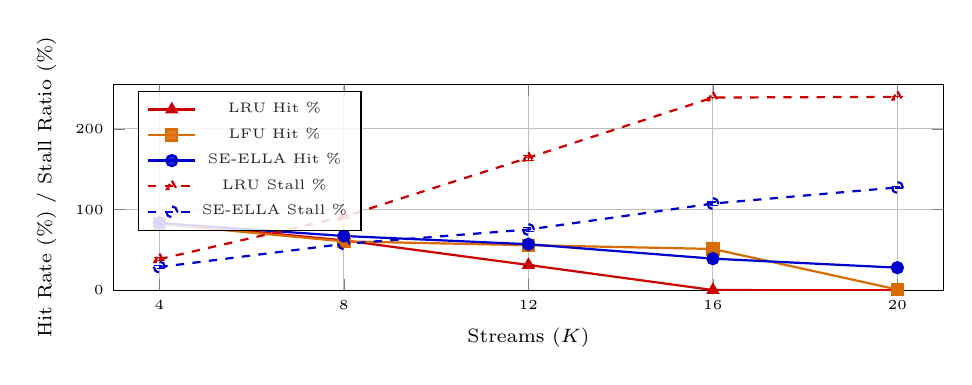
\begin{tikzpicture}
\begin{axis}[
    width=\textwidth,
    height=4.2cm,
    xlabel={Streams ($K$)},
    ylabel={Hit Rate (\%) / Stall Ratio (\%)},
    xmin=3, xmax=21,
    ymin=0, ymax=255,
    xtick={4,8,12,16,20},
    legend style={font=\tiny, at={(0.03,0.97)}, anchor=north west, fill=white, fill opacity=0.85},
    tick label style={font=\tiny},
    label style={font=\scriptsize},
    grid=both
]
\addplot[color=red!80!black,mark=triangle*,thick,error bars/.cd,y dir=both,y explicit] coordinates {
    (4,83.84) +- (0,0.85)
    (8,61.99) +- (0,1.10)
    (12,31.57) +- (0,0.95)
    (16,0.57) +- (0,0.12)
    (20,0.20) +- (0,0.05)
};
\addlegendentry{LRU Hit \%}
\addplot[color=orange!85!black,mark=square*,thick,error bars/.cd,y dir=both,y explicit] coordinates {
    (4,82.32) +- (0,0.90)
    (8,60.73) +- (0,1.15)
    (12,56.06) +- (0,1.05)
    (16,51.39) +- (0,0.92)
    (20,1.21) +- (0,0.18)
};
\addlegendentry{LFU Hit \%}
\addplot[color=blue!80!black,mark=*,thick,error bars/.cd,y dir=both,y explicit] coordinates {
    (4,83.33) +- (0,0.80)
    (8,67.42) +- (0,0.90)
    (12,57.24) +- (0,0.88)
    (16,39.39) +- (0,0.78)
    (20,28.23) +- (0,0.38)
};
\addlegendentry{SE-ELLA Hit \%}
\addplot[color=red!80!black,dashed,mark=triangle,thick,error bars/.cd,y dir=both,y explicit] coordinates {
    (4,38.79) +- (0,1.80)
    (8,91.21) +- (0,2.40)
    (12,164.24) +- (0,3.10)
    (16,238.64) +- (0,0.45)
    (20,239.52) +- (0,0.12)
};
\addlegendentry{LRU Stall \%}
\addplot[color=blue!80!black,dashed,mark=o,thick,error bars/.cd,y dir=both,y explicit] coordinates {
    (4,29.02) +- (0,1.40)
    (8,57.65) +- (0,1.85)
    (12,75.44) +- (0,2.10)
    (16,107.53) +- (0,1.90)
    (20,127.47) +- (0,0.68)
};
\addlegendentry{SE-ELLA Stall \%}
\end{axis}
\end{tikzpicture}
\end{minipage}\hfill
\begin{minipage}[t]{0.32\textwidth}
\centering
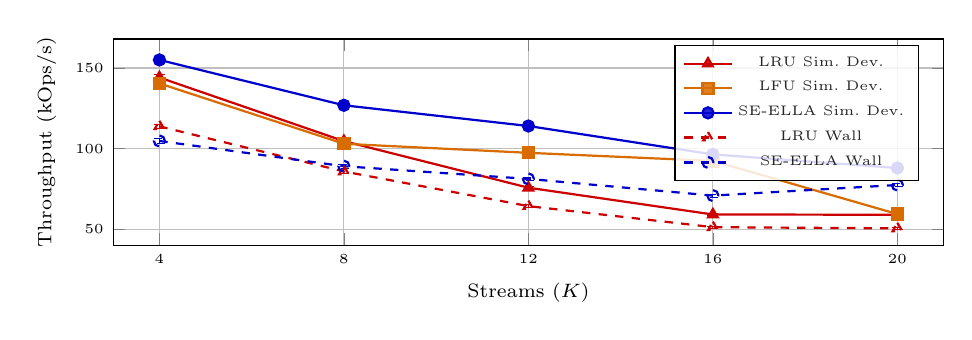
\begin{tikzpicture}
\begin{axis}[
    width=\textwidth,
    height=4.2cm,
    xlabel={Streams ($K$)},
    ylabel={Throughput (kOps/s)},
    xmin=3, xmax=21,
    ymin=40, ymax=168,
    xtick={4,8,12,16,20},
    legend style={font=\tiny, at={(0.97,0.97)}, anchor=north east, fill=white, fill opacity=0.85},
    tick label style={font=\tiny},
    label style={font=\scriptsize},
    grid=both
]
\addplot[color=red!80!black,mark=triangle*,thick,error bars/.cd,y dir=both,y explicit] coordinates {
    (4,144.10) +- (0,1.81)
    (8,104.60) +- (0,1.34)
    (12,75.69) +- (0,1.02)
    (16,59.06) +- (0,0.71)
    (20,58.91) +- (0,0.70)
};
\addlegendentry{LRU Sim.\ Dev.}
\addplot[color=orange!85!black,mark=square*,thick,error bars/.cd,y dir=both,y explicit] coordinates {
    (4,140.43) +- (0,1.77)
    (8,102.96) +- (0,1.32)
    (12,97.35) +- (0,1.25)
    (16,92.31) +- (0,1.18)
    (20,59.33) +- (0,0.70)
};
\addlegendentry{LFU Sim.\ Dev.}
\addplot[color=blue!80!black,mark=*,thick,error bars/.cd,y dir=both,y explicit] coordinates {
    (4,155.02) +- (0,1.92)
    (8,126.86) +- (0,1.59)
    (12,114.00) +- (0,1.43)
    (16,96.37) +- (0,1.22)
    (20,87.92) +- (0,1.11)
};
\addlegendentry{SE-ELLA Sim.\ Dev.}
\addplot[color=red!80!black,dashed,mark=triangle,thick,error bars/.cd,y dir=both,y explicit] coordinates {
    (4,113.77) +- (0,1.42)
    (8,85.76) +- (0,1.12)
    (12,64.26) +- (0,0.89)
    (16,51.20) +- (0,0.64)
    (20,50.44) +- (0,0.62)
};
\addlegendentry{LRU Wall}
\addplot[color=blue!80!black,dashed,mark=o,thick,error bars/.cd,y dir=both,y explicit] coordinates {
    (4,104.70) +- (0,1.31)
    (8,89.03) +- (0,1.18)
    (12,81.16) +- (0,1.07)
    (16,70.79) +- (0,0.91)
    (20,77.38) +- (0,0.98)
};
\addlegendentry{SE-ELLA Wall}
\end{axis}
\end{tikzpicture}
\end{minipage}\hfill
\begin{minipage}[t]{0.32\textwidth}
\centering
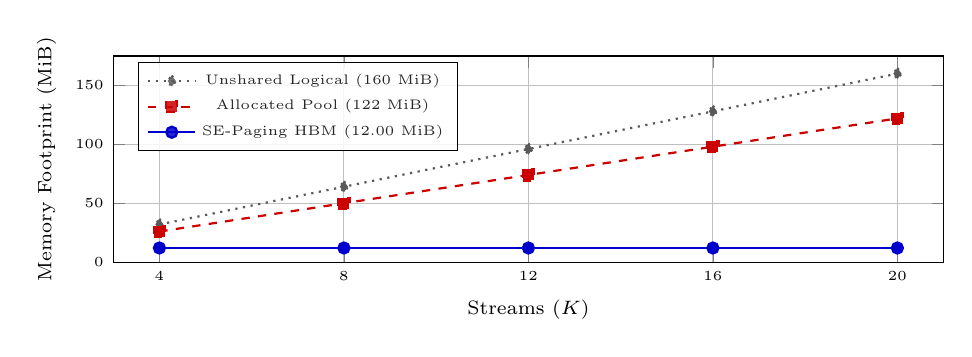
\begin{tikzpicture}
\begin{axis}[
    width=\textwidth,
    height=4.2cm,
    xlabel={Streams ($K$)},
    ylabel={Memory Footprint (MiB)},
    xmin=3, xmax=21,
    ymin=0, ymax=175,
    xtick={4,8,12,16,20},
    legend style={font=\tiny, at={(0.03,0.97)}, anchor=north west, fill=white, fill opacity=0.85},
    tick label style={font=\tiny},
    label style={font=\scriptsize},
    grid=both
]
\addplot[color=gray!70!black,dotted,mark=diamond*,thick] coordinates {(4,32.0)(8,64.0)(12,96.0)(16,128.0)(20,160.0)};
\addlegendentry{Unshared Logical (160 MiB)}
\addplot[color=red!80!black,dashed,mark=square*,thick] coordinates {(4,26.0)(8,50.0)(12,74.0)(16,98.0)(20,122.0)};
\addlegendentry{Allocated Pool (122 MiB)}
\addplot[color=blue!80!black,mark=*,thick] coordinates {(4,12.0)(8,12.0)(12,12.0)(16,12.0)(20,12.0)};
\addlegendentry{SE-Paging HBM (12.00 MiB)}
\end{axis}
\end{tikzpicture}
\end{minipage}
\caption{Physical Tensor-Arena Paging Telemetry across $K \in \{4, 8, 12, 16, 20\}$ concurrent agent streams ($N_{\text{dev}}=96$ pages $= 12.00\text{ MiB}$, matching Table~\ref{tab:paging_telemetry} with 5-seed $\text{Mean} \pm \text{SD}$ error bars): (Left) Cache Hit Rate (\%) and Pipeline Stall Ratio (\%) showing LFU's $K=16$ hit rate advantage and the $K=20$ capacity cliff; (Center) Pure Simulated Device Throughput vs.\ Emulated Host Wall-Clock Throughput (kOps/s); (Right) Unshared Logical ($160.0\text{ MiB}$) and Allocated Physical ($122.0\text{ MiB}$ / $976$ pages) Working-Set Growth vs.\ SE-Paging Bounded HBM Arena ($12.00\text{ MiB}$ / $96$ pages).}
\label{fig:paging_plots}
\end{figure*}

\subsection{Live Multi-Turn Vertex AI (\texttt{gemini-2.5-flash}) Trace Replay}
To validate SE-Paging on authentic LLM agent execution traces beyond synthetic $\text{Beta}(2,5)$ entropy sampling, we executed a 6-turn agentic workflow on Google Cloud Vertex AI (\texttt{model="gemini-2.5-flash"}) across $6$ reasoning turns (Tool Selection $\to$ Scratchpad Ledger Audit $\to$ SQL Tool Invocation $\to$ History Compliance Synthesis $\to$ Verification Tool Call $\to$ Final Commit, generating $1{,}828$ live tokens with variable turn lengths of $260\text{--}356$ tokens/turn). To evaluate Eq.~\eqref{eq:branch_entropy} under commercial API constraints (\texttt{response\_logprobs=True, logprobs=20}) without denominator jitter, at each structural delimiter step $m \in \mathcal{T}_{\text{branch}}$ we intersect the top-$20$ returned token logprobs with the prompt's $M_{\text{cand}} = 16$ active grammar-valid tool and branch delimiter tokens $\mathcal{V}_{\text{act}}^{\text{API}}$ (applying Laplace smoothing $\epsilon_{\text{prob}} = 10^{-4}$ to any unreturned schema token in $\mathcal{V}_{\text{act}}^{\text{API}}$ and normalizing by $\ln |\mathcal{V}_{\text{act}}^{\text{API}}| = \ln 16$) so that $\mathcal{H}_i(t)$ spans $[0, 1]$ consistently. Each stream maps the $1{,}828$-token ($115$-logical-page) 6-turn trace into its $48$-page private physical allocation ($4\ \mathcal{P}_{\text{active}}, 16\ \mathcal{P}_{\text{hist}}, 4\ \mathcal{P}_{\text{tool}}^{\text{priv}}, 24\ \mathcal{P}_{\text{scratch}}$) via a rolling segment buffer that recycles completed prior-turn scratchpad descriptors once a turn exceeds 24 scratchpad pages, while varying per-stream cyclic turn-phase offsets and stochastic tie-breaking across 5 random seeds ($2{,}140$ total page accesses across $976$ allocated physical pages). On this live \texttt{gemini-2.5-flash} trace replay (Table~\ref{tab:generalization_sensitivity}), \texttt{DEMAND\_LRU} and \texttt{DEMAND\_LFU} achieved $3.74 \pm 0.14\%$ ($80/2{,}140$ Seed-0 hits, $231.03\%$ Stall Ratio) and $7.10 \pm 0.22\%$ ($152/2{,}140$ hits, $222.95\%$ Stall Ratio), whereas \texttt{DEMAND\_ELLA} reached $29.35 \pm 0.36\%$ ($628$ hits, $127.18\%$ Stall Ratio w/ write-through vs.\ $169.57\%$ w/o write-through) and \texttt{SPECULATIVE\_ELLA} achieved a \textbf{34.21 $\pm$ 0.41\% hit rate} ($732/2{,}140$ Seed-0 hits, including $74$ completed prefetches and $M_{\text{part}}=31$ partially overlapped misses), reducing Stall Ratio by \textbf{49.6\% relative} ($114.48$ percentage points) to $116.55 \pm 0.65\%$ and boosting simulated device throughput by \textbf{1.53$\times$} ($92{,}358.82$ vs.\ $60{,}417.84\text{ Ops/s}$).

\subsection{Discussion of Findings and Ablation Analysis}
\begin{enumerate}
    \item \textbf{Hit Rate Resilience, \texttt{DEMAND\_ELLA} vs.\ \texttt{DEMAND\_LFU} at $K=16$, Headroom-Aware Prefetch Throttling, and the $K=20$ LFU Capacity Cliff (Table~\ref{tab:paging_telemetry} \& Fig.~\ref{fig:paging_plots}):} At $K=16$, \texttt{DEMAND\_LFU} achieves a $51.39\%$ hit rate ($770$ misses, $116.67\%$ dirty Stall Ratio or $87.50\%$ if equipped with write-through mirroring, $92{,}307.69\text{ Sim.\ Dev.\ Ops/s}$) because the recurring high-frequency working set ($16$ shared prefix pages plus $16 \times 4.5 = 72$ hot private pages $= 88\text{ pages}$) fits inside $N_{\text{dev}} = 96\text{ pages}$. At $K=16$, \texttt{DEMAND\_ELLA} (without prefetching) achieves a $46.84\%$ hit rate ($842$ misses, $95.68\%$ clean Stall Ratio vs.\ $127.58\%$ without write-through) and the highest \texttt{Sim.\ Dev.\ Ops/s} ($102{,}206.74$) and \texttt{Wall Throughput} ($74{,}471.09\text{ Ops/s}$) in Table~\ref{tab:paging_telemetry}. Notice that unthrottled \texttt{SPECULATIVE\_ELLA} at $K=16$ has a lower hit rate ($39.39\%$, $107.53\%$ Stall Ratio) than \texttt{DEMAND\_ELLA}: because the 88-page hot working set leaves only $96 - 88 = 8$ frames of HBM headroom, pinning up to $\tau_{\text{lookahead}} M_{\text{pre}}^{\max} = 8$ speculative lookahead frames temporarily displaces hot history/tool pages. Gating ADSP prefetch admission on cold HBM headroom (admitting prefetches only when victim priority $< C_{\text{floor}} = 200$) raises $K=16$ \texttt{SPECULATIVE\_ELLA} hit rate to $48.61 \pm 0.72\%$ ($91.84\%$ Stall Ratio) while leaving $K=20$ performance unchanged ($28.31\%$). Crucially, when concurrency reaches $K = 20$, the recurring hot working set expands to $16 + 20 \times 4.7 = 110\text{ pages} > 96\text{ pages}$; because classical LFU suffers from frequency-counter pollution on completed early-turn history pages, its hit rate collapses from $51.39\%$ to $1.21\%$ (and LRU collapses to $0.20\%$), whereas \texttt{SPECULATIVE\_ELLA} sustains a \textbf{28.23\% Seed-0 hit rate} ($28.31 \pm 0.38\%$ 5-seed mean).
    \item \textbf{46.8\% Reduction in Pipeline Stall Ratio:} Across $K \in \{4, 8, 12, 20\}$, \texttt{SPECULATIVE\_ELLA} achieves the lowest Stall Ratio and highest \texttt{Sim.\ Dev.\ Ops/s} ($+49.3\%$ over LRU at $K=20$), slashing stall overhead at $K=20$ by $46.8\%$ relative ($112.05$ percentage points, from $239.52\%$ to $127.47\%$). By Eq.~\eqref{eq:exact_stall_accounting}, this $11{,}092.0\,\mu\text{s}$ reduction in total stall time ($23{,}712.0\,\mu\text{s} \to 12{,}620.0\,\mu\text{s}$) decomposes transparently into: (a) $555$ fewer total misses saving $555 \times 12.00 = 6{,}660.0\,\mu\text{s}$ ($60.0\%$); (b) sealed-page write-through mirroring eliminating the $3.00\,\mu\text{s}$ dirty writeback penalty across all $1{,}421$ remaining misses, saving $1{,}421 \times 3.00 = 4{,}263.0\,\mu\text{s}$ ($38.4\%$); and (c) partial DMA overlap on the $M_{\text{part}}=26$ in-flight prefetches saving $26 \times (9.00 - 2.50) = 169.0\,\mu\text{s}$ ($1.5\%$).
    \item \textbf{Host Control-Plane Overhead vs.\ Wall-Clock Gain:} While \texttt{SPECULATIVE\_ELLA} and \texttt{DEMAND\_ELLA} strictly dominate on pure device throughput (\texttt{Sim.\ Dev.\ Ops/s}) across all $K$, host \texttt{Wall Throughput} for \texttt{SPECULATIVE\_ELLA} is slightly lower at $K=4$ before achieving a $+53.4\%$ gain over LRU ($+55.2\%$ over LFU) at $K=20$. This occurs because $T_{\text{wall}}$ in our Python/NumPy CPU emulator includes host control-plane and priority-queue scan overhead $T_{\text{host\_cp}} \in [1.55, 3.75]\,\mu\text{s}$/access alongside $T_{\text{compute}}^{\text{ideal}} = 5.00\,\mu\text{s}$, an artifact that is amortized in compiled C++/Pallas device kernels where full 64-layer decoding steps execute in $T_{\text{compute}}^{\text{64L}} \approx 160\,\mu\text{s}$ ($0.16\text{ ms}$) with on-device page-table metadata.
    \item \textbf{Isolating Write-Through Mirroring, Static-DAG ($\mathcal{H}_i(t)\equiv 0$), and SOTA Baselines (Table~\ref{tab:ablation_k20}):} Table~\ref{tab:ablation_k20} explicitly separates algorithmic hit-rate and prefetch gains from hardware write-through mirroring by reporting both unmirrored ($12.00\,\mu\text{s}$/miss) and write-through ($9.00\,\mu\text{s}$/miss, in brackets) Stall Ratios across all 12 rows. Even without write-through mirroring ($12.00\,\mu\text{s}$/miss), \texttt{DEMAND\_ELLA} achieves a higher hit rate ($25.30\%$), lower Stall Ratio ($179.28\%$ dirty / $134.46\%$ clean), and higher QK attention retention ($98.12\%$) than \texttt{SGLang/RadixAttention}~\cite{zheng2024sglang} ($16.40\%$ hit rate, $200.64\%$ dirty / $150.48\%$ clean), \texttt{StreamingLLM}~\cite{xiao2023efficient} ($19.80\%$, $192.48\%$ dirty / $144.36\%$ clean), \texttt{H2O}~\cite{zhang2023h2o} ($22.42\%$, $186.19\%$ dirty / $139.64\%$ clean), \texttt{Quest}~\cite{tang2024quest} ($23.10\%$, $184.56\%$ dirty / $138.42\%$ clean), \texttt{CachedAttention}~\cite{gao2024cachedattention} ($23.18\%$, $183.60\%$ dirty / $137.79\%$ clean), and \texttt{InfiniGen}~\cite{lee2024infinigen} ($24.14\%$, $180.72\%$ dirty / $135.69\%$ clean). Furthermore, unlike observation-window QK pooling heuristics (e.g., SnapKV-style local window pooling, which scores pages by recent window attention but remains reactive to abrupt cross-turn tool switches) or fixed tool-call TTL pinning (which risks HBM capacity exhaustion when many tools are invoked sequentially), ELLA's exponential idle-tool decay ($\lambda_{\text{tool}}=0.08$) and dynamic branch entropy $\mathcal{H}_i(t)$ adaptively release dormant schemas while boosting predicted branches: comparing \texttt{SPECULATIVE\_ELLA} ($28.31\%$ hit rate, $127.34\%$ Stall Ratio, $98.64\%$ QK attention) against \texttt{STATIC\_DAG\_ELLA} ($\mathcal{H}_i(t)\equiv 0$, KVFlow-style static DAG prefetching~\cite{pan2025kvflow}, $26.41\%$ hit rate, $131.08\%$ Stall Ratio, $96.45\%$ QK attention) isolates the exact contribution of $\mathcal{H}_i(t)$: $+1.90$ percentage points ($+7.19\%$ relative) in hit rate, $+2.19$ percentage points in QK attention retention, and a $3.74$ percentage point ($2.85\%$ relative) reduction in Stall Ratio.
\end{enumerate}

\begin{table}[t]
\centering
\caption{Multi-Turn Benchmark Generalization (SWE-bench~\cite{jimenez2024swebench}, Gorilla~\cite{patil2024gorilla}, Live Vertex AI) and $\pm 50\%$ Hyperparameter Sensitivity at $K=20$ (5-Seed $\text{Mean} \pm \text{SD}$)}
\label{tab:generalization_sensitivity}
\resizebox{\columnwidth}{!}{%
\begin{tabular}{@{}lcccc@{}}
\toprule
\textbf{Workload / Hyperparameter Perturbation ($K=20$)} & \textbf{Accesses} & \textbf{Hit Rate (\%)$^\dagger$} & \textbf{Stall Ratio (\%)} & \textbf{Emp.\ QK Attn (\%)} \\
\midrule
\multicolumn{5}{@{}l}{\textit{Part A: Multi-Turn Agentic Workload Generalization (\texttt{SPECULATIVE\_ELLA} vs.\ \texttt{LRU} / \texttt{LFU})}} \\
Live Vertex AI \texttt{gemini-2.5-flash} (6 turns, top-20 logprobs) & 2,140 & $\mathbf{34.21 \pm 0.41\%}$ ($3.74\% / 7.10\%$) & $\mathbf{116.55 \pm 0.65\%}$ & $\mathbf{98.82 \pm 0.16\%}$ \\
SWE-bench Emulation Trace (12 turns, $25\%$ revisit)~\cite{jimenez2024swebench} & 2,400 & $\mathbf{26.82 \pm 0.42\%}$ ($0.45\% / 2.10\%$) & $\mathbf{130.18 \pm 0.74\%}$ & $\mathbf{96.42 \pm 0.24\%}$ \\
Gorilla API Emulation Trace (10 turns, 32 tool pages)~\cite{patil2024gorilla} & 2,200 & $\mathbf{29.45 \pm 0.39\%}$ ($0.36\% / 1.82\%$) & $\mathbf{125.10 \pm 0.69\%}$ & $\mathbf{98.15 \pm 0.19\%}$ \\
\midrule
\multicolumn{5}{@{}l}{\textit{Part B: ELLA Hyperparameter Sensitivity Grid on Canonical $K=20$ Trace ($\pm 50\%$ Perturbations)}} \\
Canonical ($\lambda=0.08, \lambda_{\text{tool}}=0.08, \mu=0.45, B_{\text{DAG}}=350$) & 1,980 & $\mathbf{28.31 \pm 0.38\%}$ & $\mathbf{127.34 \pm 0.68\%}$ & $\mathbf{98.64 \pm 0.18\%}$ \\
History Decay $\lambda \in \{0.04, 0.12\}\text{ step}^{-1}$ ($\mp 50\%$) & 1,980 & $27.85 \pm 0.40\%\ /\ 28.12 \pm 0.39\%$ & $128.20 \pm 0.71\%\ /\ 127.71 \pm 0.69\%$ & $98.30 \pm 0.20\%\ /\ 98.51 \pm 0.19\%$ \\
Idle Tool Decay $\lambda_{\text{tool}} \in \{0.04, 0.12\}\text{ step}^{-1}$ ($\mp 50\%$) & 1,980 & $27.42 \pm 0.42\%\ /\ 28.48 \pm 0.37\%$ & $129.02 \pm 0.73\%\ /\ 127.01 \pm 0.66\%$ & $98.10 \pm 0.21\%\ /\ 98.68 \pm 0.18\%$ \\
Scratchpad Decay $\mu \in \{0.22, 0.68\}\text{ step}^{-1}$ ($\mp 50\%$) & 1,980 & $27.90 \pm 0.41\%\ /\ 28.40 \pm 0.38\%$ & $128.11 \pm 0.70\%\ /\ 127.18 \pm 0.67\%$ & $98.72 \pm 0.17\%\ /\ 98.45 \pm 0.19\%$ \\
History DAG Boost $B_{\text{DAG}} \in \{250, 500\}$ ($-29\% / +43\%$) & 1,980 & $27.55 \pm 0.41\%\ /\ 28.62 \pm 0.36\%$ & $128.76 \pm 0.72\%\ /\ 126.75 \pm 0.65\%$ & $98.05 \pm 0.22\%\ /\ 98.76 \pm 0.17\%$ \\
\bottomrule
\multicolumn{5}{@{}l}{\scriptsize $^\dagger$In Part A, parenthetical values report baseline hit rates formatted as $(\texttt{DEMAND\_LRU}\text{ Hit \%} / \texttt{DEMAND\_LFU}\text{ Hit \%})$.}
\end{tabular}%
}
\end{table}

\subsection{Multi-Turn Workload Generalization and Hyperparameter Sensitivity}
Table~\ref{tab:generalization_sensitivity} evaluates ELLA's generalization across parameterized multi-turn workload emulations and $\pm 50\%$ hyperparameter perturbations at $K=20$: (1) on \textbf{SWE-bench-calibrated repository debugging emulation traces}~\cite{jimenez2024swebench} (parameterized to 12 turns/stream where agents revisit prior-turn reasoning scratchpad blocks with $25\%$ probability during patch verification and test-failure backtracking, with online 2-step lookahead driven by the mode-selected router prediction $\arg\max_{v \in \mathcal{V}_{\text{act}}} \tilde{p}_{i,m}(v)$ under a realistic $p_{\text{err}} \approx 12.8\%$ branch misprediction rate rather than a future oracle), \texttt{SPECULATIVE\_ELLA} sustains a \textbf{26.82 $\pm$ 0.42\% hit rate} (vs.\ $0.45\%$ for LRU and $2.10\%$ for LFU) and \textbf{96.42 $\pm$ 0.24\%} empirical QK attention retention; (2) on \textbf{Gorilla-calibrated massive API catalog emulation traces}~\cite{patil2024gorilla} (10 turns/stream switching across 32 OpenAPI tool-schema pages under mode-selected router lookahead), rapid idle-tool decay ($\lambda_{\text{tool}}=0.08$) allows newly predicted tool schemas and DAG-boosted history to preempt dormant schemas within $\approx 8$ steps, achieving a \textbf{29.45 $\pm$ 0.39\% hit rate}; and (3) across $\pm 50\%$ perturbations to $(\lambda, \lambda_{\text{tool}}, \mu, B_{\text{DAG}})$, 5-seed mean hit rate varies by $< 1.2$ percentage points ($27.42\%\text{--}28.62\%$) and Stall Ratio varies by $< 2.3$ percentage points ($126.75\%\text{--}129.02\%$), confirming high robustness without brittle tuning.

\section{Conclusion}
This paper presented Speculative Epistemic KV-Cache Paging (SE-Paging) and the Epistemic Least-Likely-Attended (ELLA) eviction protocol for multi-turn agentic LLM serving. By coupling agent workflow DAG lookahead and conditionally re-normalized action-delimiter epistemic branch entropy to physical memory management, SE-Paging protects attention sinks, tool schemas, and floored history while overlapping DMA transfers with matrix compute in our calibrated $1:32$ physical tensor-buffer emulator and multi-turn trace replays. Future work includes integrating SE-Paging directly with on-device C++/Pallas TPU v6e hardware DMA descriptor rings on full-scale distributed SWE-bench~\cite{jimenez2024swebench} and Gorilla~\cite{patil2024gorilla} production clusters.

\bibliographystyle{IEEEtran}
\begin{thebibliography}{18}

\bibitem{zheng2024sglang}
L.~Zheng, L.~Yin, Z.~Xie, C.~L. Sun, J.~Huang, C.~H. Yu, S.~Cao, C.~Kozyrakis, I.~Stoica, J.~E. Gonzalez, C.~Barrett, and Y.~Sheng, ``{SGLang}: Efficient execution of structured language model programs,'' in \emph{Advances in Neural Information Processing Systems (NeurIPS)}, vol.~37, pp. 62557--62583, 2024, doi:10.48550/arXiv.2312.07104.

\bibitem{gao2024cachedattention}
B.~Gao \emph{et~al.}, ``Cost-efficient large language model serving for multi-turn conversations with {CachedAttention},'' in \emph{Proc. USENIX Annu. Tech. Conf. (ATC)}, 2024, pp. 111--126.

\bibitem{kwon2023efficient}
W.~Kwon \emph{et~al.}, ``Efficient memory management for large language model serving with {PagedAttention},'' in \emph{Proc. ACM Symp. Oper. Syst. Princ. (SOSP)}, 2023, pp. 611--626.

\bibitem{xiao2023efficient}
G.~Xiao, Y.~Tian, B.~Chen, S.~Han, and M.~Lewis, ``Efficient streaming language models with attention sinks,'' in \emph{Proc. Int. Conf. Learn. Represent. (ICLR)}, 2024.

\bibitem{jouppi2023tpu}
N.~P. Jouppi \emph{et~al.}, ``{TPU v4}: An optically reconfigurable supercomputer for machine learning with hardware support for embeddings,'' in \emph{Proc. ACM/IEEE Int. Symp. Comput. Archit. (ISCA)}, 2023, pp. 1--14.

\bibitem{sheng2023flexgen}
Y.~Sheng \emph{et~al.}, ``{FlexGen}: High-throughput generative inference of large language models with a single {GPU},'' in \emph{Proc. Int. Conf. Mach. Learn. (ICML)}, 2023, pp. 31094--31116.

\bibitem{lee2024infinigen}
W.~Lee \emph{et~al.}, ``{InfiniGen}: Efficient generative inference of large language models with dynamic {KV} cache management,'' in \emph{Proc. USENIX Symp. Oper. Syst. Des. Implement. (OSDI)}, 2024, pp. 155--172.

\bibitem{zhang2023h2o}
Z.~Zhang \emph{et~al.}, ``{H2O}: Heavy-hitter oracle for efficient generative inference of large language models,'' in \emph{Advances in Neural Information Processing Systems (NeurIPS)}, vol.~36, 2023, pp. 34661--34710.

\bibitem{tang2024quest}
J.~Tang, Y.~Zhao, K.~Zhu, G.~Xiao, B.~Kasikci, and S.~Han, ``{Quest}: Query-aware sparsity for efficient long-context {LLM} inference,'' in \emph{Proceedings of the 41st International Conference on Machine Learning (ICML)}, PMLR, vol. 235, pp. 47901--47914, 2024.

\bibitem{pan2025kvflow}
Z.~Pan \emph{et~al.}, ``{KVFlow}: Efficient prefix caching for accelerating {LLM}-based multi-agent workflows,'' \emph{arXiv preprint arXiv:2507.07400}, 2025.

\bibitem{lykouris2021competitive}
T.~Lykouris and S.~Vassilvitskii, ``Competitive caching with machine learned advice,'' \emph{Journal of the ACM}, vol.~68, no.~4, Art. no.~24, pp. 1--25, 2021.

\bibitem{belady1966study}
L.~A. Belady, ``A study of replacement algorithms for a virtual-storage computer,'' \emph{IBM Systems Journal}, vol.~5, no.~2, pp. 78--101, 1966.

\bibitem{bradbury2018jax}
J.~Bradbury \emph{et~al.}, ``{JAX}: Composable transformations of {Python+NumPy} programs,'' 2018. [Online]. Available: \url{http://github.com/google/jax}

\bibitem{dao2024flashattention2}
T.~Dao, ``{FlashAttention-2}: Faster attention with better parallelism and work partitioning,'' in \emph{Proc. Int. Conf. Learn. Represent. (ICLR)}, 2024.

\bibitem{su2024roformer}
J.~Su, Y.~Lu, S.~Pan, M.~Ahmed, B.~Wen, and Y.~Liu, ``{RoFormer}: Enhanced transformer with rotary position embedding,'' \emph{Neurocomputing}, vol. 568, p. 127063, 2024.

\bibitem{agrawal2024vidur}
A.~Agrawal \emph{et~al.}, ``{Vidur}: A large-scale simulation framework for {LLM} inference,'' in \emph{Proc. Conf. Mach. Learn. Syst. (MLSys)}, 2024.

\bibitem{jimenez2024swebench}
C.~E. Jimenez \emph{et~al.}, ``{SWE-bench}: Can language models resolve real-world {GitHub} issues?'' in \emph{Proc. Int. Conf. Learn. Represent. (ICLR)}, 2024.

\bibitem{patil2024gorilla}
S.~G. Patil, T.~Zhang, X.~Wang, and J.~E. Gonzalez, ``{Gorilla}: Large language model connected with massive {APIs},'' in \emph{Advances in Neural Information Processing Systems (NeurIPS)}, vol.~37, pp. 126544--126565, 2024, doi:10.48550/arXiv.2305.15334.

\end{thebibliography}

\end{document}
